\chapter{Desarrollo de la extensión de la herramienta}\label{chapter:desarrollo}

\section{Análisis de requisitos}

En esta sección se presenta un análisis detallado de los requisitos del proyecto cuyo objetivo es ayudar a los ingenieros de software a desarrollar sistemas IoT, automatizando parte de sus tareas mediante la extensión de la herramienta TDDT4IoTS. Se han identificado y categorizado los requisitos funcionales y no funcionales, así como las restricciones y los recursos utilizados. La solución propuesta utiliza modelos entrenados de OpenAI, específicamente el modelo base GPT-3.5-Turbo, para analizar las descripciones de los casos de uso y generar automáticamente estructuras JSON que representan diagramas de clases.

%En esta sección se presenta un análisis de los requisitos del proyecto que busca asistir a los ingenieros de software en el desarrollo de sistemas IoT mediante la automatización de ciertas tareas. Para lograrlo, se propone la extensión de la herramienta TDDT4IoTS, dotándola de capacidades avanzadas basadas en inteligencia artificial. La solución implica el uso de modelos de IA para analizar descripciones de casos de uso y generar estructuras JSON, que luego se utilizarán para crear diagramas de clases. Este análisis es fundamental para garantizar que todas las necesidades y limitaciones del proyecto sean comprendidas y abordadas adecuadamente.

El propósito de esta sección es proporcionar una visión clara de los diferentes tipos de requisitos necesarios para el desarrollo del sistema, incluyendo los funcionales y no funcionales, así como las restricciones y los recursos utilizados. Esta comprensión detallada asegurará que el proyecto se desarrolle de manera efectiva, cumpliendo con las expectativas de los usuarios y los objetivos del proyecto.

\subsection{Requisitos funcionales}

Los requisitos funcionales se utiliza para para definir las capacidades y características específicas que debe tener el sistema para cumplir con los objetivos del proyecto. Un aspecto clave es la identificación automática de elementos clave a partir de descripciones textuales proporcionadas por los desarrolladores. Esto incluye la capacidad de detectar clases, atributos y relaciones dentro del sistema descrito, facilitando así la generación inicial de los diagramas de clases conceptuales.

Otra funcionalidad es la capacidad de generar el grafico correspondiente al diagrama de clases a partir de las estructura JSON generada a partir del análisis de las descripciones de los casos de uso. Este diagrama será el esquema inicial del proyecto, proporcionando una base que los ingenieros pueden refinar posteriormente para obtener diagramas de clases del dominio de la solución. Además, la herramienta extendida debe integrarse sin problemas con TDDT4IoTS, permitiendo a los usuarios (ingenieros en software) aprovechar las nuevas funcionalidades para facilitar su labor y aumentar su productividad.

\subsection{Requisitos No Funcionales}

Los requisitos no funcionales se refieren a los criterios que deben cumplir los sistemas en términos de:

\begin{itemize}
	\item \textbf{Rendimiento y eficiencia:}
	El sistema debe ser capaz de procesar descripciones textuales y generar diagramas de clases de manera rápida y eficiente, para minimizar el tiempo de espera de los usuarios. La integración de los modelos de IA debe estar optimizada para asegurar tiempos de respuesta aceptables, incluso bajo cargas de trabajo altas.
	
	\item \textbf{Usabilidad:}
	La interfaz del sistema debe ser intuitiva y fácil de usar, permitiendo que los ingenieros de software aprovechen las nuevas funcionalidades sin una curva de aprendizaje pronunciada. Esto incluye una interfaz gráfica clara, guías de usuario y documentación accesible.
	
	\item \textbf{Fiabilidad:}
	El sistema debe ser estable y confiable, asegurando un tiempo de inactividad mínimo y una alta disponibilidad para los usuarios. Debe ser capaz de manejar errores de manera robusta y recuperar su estado normal sin pérdida de datos.
	
	\item \textbf{Mantenibilidad:}
	El sistema debe estar diseñado de manera que sea fácil de mantener y actualizar. Esto incluye una arquitectura modular que permita realizar mejoras y correcciones de errores sin afectar el funcionamiento general del sistema. La documentación del código debe ser clara y completa para facilitar su mantenimiento.
	
	\item \textbf{Escalabilidad:}
	La arquitectura del sistema debe permitir la escalabilidad para manejar un creciente número de usuarios y la cantidad de datos procesados sin degradar el rendimiento del sistema. Esto incluye la capacidad de distribuir la carga de trabajo y aumentar la capacidad del sistema según sea necesario.
\end{itemize}

\subsection{Restricciones}

Las restricciones del proyecto son los factores que limitan las opciones de diseño y desarrollo, imponiendo ciertos límites que deben ser respetados.

\begin{itemize}
	\item \textbf{Dependencia de servicios de IA:}
	La solución depende del uso de la API de servicios de OpenAI, lo cual implica un costo asociado y posibles limitaciones en la disponibilidad del servicio. Es crucial gestionar adecuadamente los costos y tener planes de contingencia para posibles interrupciones del servicio.
	
	\item \textbf{Licencias de software \textit{open source}:}
	Todo el software \textit{open source} utilizado debe cumplir con sus respectivas licencias, asegurando que no se infrinjan derechos de propiedad intelectual. Es importante revisar y entender las condiciones de cada licencia para evitar problemas legales.
	
	\item \textbf{Integración con sistemas existentes:}
	La herramienta implementada debe integrarse sin problemas con la herramienta TDDT4IoTS existente y otros sistemas de apoyo. Esto puede requerir adaptaciones específicas para asegurar la compatibilidad y un funcionamiento fluido entre los diferentes componentes del sistema resultante.
\end{itemize}

\subsection{Recursos Utilizados}

Los recursos utilizados para el desarrollo del proyecto incluyen tanto herramientas de software como servicios externos, para lograr los objetivos propuestos.

\begin{itemize}
	\item \textbf{Modelos de IA:}
	Utilización de modelos de IA para procesar texto y extraer información relevante. Los modelos pueden ser seleccionados y configurados según las necesidades del desarrollador, optimizando así el proceso de diseño de sistemas.
	
	\item \textbf{Framework Spring:}
	Uso de Spring para el desarrollo de microservicios que gestionan las funcionalidades del sistema y la comunicación con la base de datos PostgreSQL. Spring Boot proporciona una plataforma robusta y escalable para construir aplicaciones empresariales.
	
	\item \textbf{PostgreSQL:}
	Base de datos relacional utilizada para almacenar la información relevante del sistema, como descripciones textuales, estructuras JSON generadas y diagramas de clases. PostgreSQL es conocido por su fiabilidad y rendimiento, siendo adecuado para aplicaciones de misión crítica.
	
	\item \textbf{gRPC:}
	Protocolo de comunicación utilizado para la interacción eficiente entre los microservicios de Spring y el componente de Python que maneja la integración con la API de servicios de inteligencia artificial. gRPC permite una comunicación rápida y eficiente para aplicaciones distribuidas.
	
	\item \textbf{HTTPS:}
	Protocolo utilizado para la comunicación entre el servicio de gestión de usuarios y el servidor existente de la herramienta, validando las peticiones mediante tokens de sesión. HTTPS es ampliamente utilizado y proporciona un medio estándar para la comunicación en la web.
\end{itemize}

\section{Arquitectura}

La arquitectura del sistema desarrollado para la extensión de la herramienta TDDT4IoTS está diseñada para ser modular, escalable y fácil de mantener. Esta arquitectura se compone de varias capas, cada una con responsabilidades específicas, lo que permite una clara separación de preocupaciones y facilita tanto el desarrollo como la integración de nuevas funcionalidades. La estructura en capas asegura que cada componente del sistema pueda evolucionar independientemente, mejorando la robustez y la flexibilidad del mismo.

\begin{figure}[H]  
	\centering
	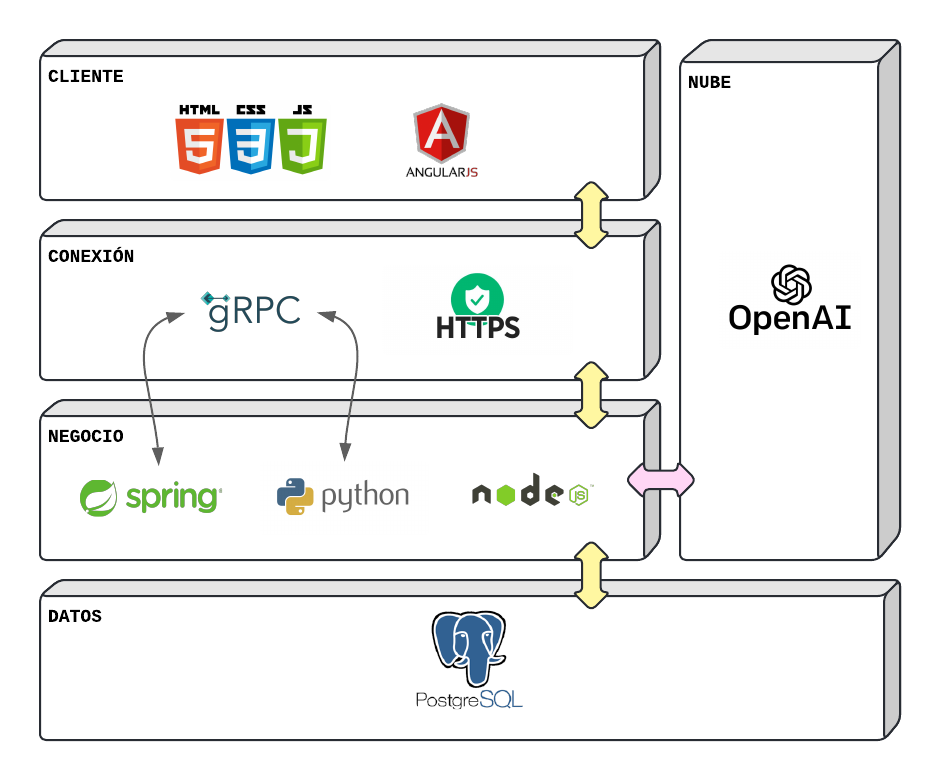
\includegraphics[width=300px]{cap3_arquitectura.png}
	\caption{Arquitectura de la extensión.}
	\label{fig:cap3_arquitectura}
\end{figure}

La figura \ref{fig:cap3_arquitectura} presenta las tecnologías utilizadas en las diferentes capas que componen la arquitectura del sistema: la capa del cliente, la capa de conexión, la capa de negocio, la capa de la nube y la capa de datos, describiéndose cada una de ellas en los siguientes subapartados que se incluyen a continuación. Cada una de estas capas juega un papel importante en el funcionamiento del sistema, asegurando que las interacciones entre los usuarios y las funcionalidades avanzadas basadas en inteligencia artificial se realicen de manera eficiente y segura. Esta organización en capas también facilita la gestión de la lógica del negocio, el almacenamiento de datos y la comunicación entre los diferentes servicios que forman parte de la solución.


\subsection{Capa del cliente}

La capa del cliente es la interfaz donde los usuarios interactúan directamente con la herramienta y la extensión implementada. Esta capa se encarga de proporcionar una experiencia de usuario intuitiva y accesible mediante interfaces web. Los usuarios pueden acceder a las funcionalidades de la herramienta, como la creación y análisis de casos de uso, y visualizar los diagramas de clases generados. Esta capa incluye todas las vistas y componentes de la interfaz de usuario que permiten a los ingenieros de software realizar sus tareas de manera eficiente.

\begin{itemize}
	\item \textbf{Interfaces web:} Desarrolladas utilizando tecnologías como HTML, CSS y JavaScript, junto con frameworks modernos como React o Angular, estas interfaces permiten a los usuarios interactuar con las funcionalidades de la herramienta.
	\item \textbf{Interacción usuario-sistema:} Los usuarios pueden enviar descripciones de casos de uso, recibir los resultados del análisis efectuado y gestionar sus proyectos directamente desde el navegador web.
\end{itemize}

\subsection{Capa de conexión}

La capa de conexión se encarga de manejar las comunicaciones entre los diferentes componentes del sistema. Esta capa es crucial para garantizar que los datos fluyan de manera eficiente y segura entre las diferentes partes del sistema.

\begin{itemize}
	\item \textbf{Conexión HTTPS:} Utilizada para la comunicación entre el cliente y la capa de negocio. Las peticiones HTTPS son manejadas por el \textit{framework} Spring, que gestiona la validación de las solicitudes y la entrega de respuestas adecuadas.
	\item \textbf{Conexión gRPC:} Establece la conexión entre los microservicios implementados con Spring y Python que se encuentran en la capa de negocio, y que manejan la integración con los modelos de IA. gRPC proporciona una comunicación rápida y eficiente, esencial para el procesamiento intensivo de datos requerido por los modelos de IA.
\end{itemize}

\subsection{Capa de negocio}

La capa de negocio alberga todos los microservicios implementados que contienen la lógica del negocio necesaria para manejar el uso de los modelos de inteligencia artificial y el entrenamiento de los mismos. Esta capa es el núcleo funcional de la aplicación, donde se llevan a cabo las principales operaciones.

\begin{itemize}
	\item \textbf{Microservicios:} Para el control de todas las peticiones que son enviadas por el cliente se desarrollaron los microservicios con Spring Boot. Python fue implementado de forma interna para controlar las peticiones que se realizarían con la API de OpenAI, comunicándose igualmente mediante gRPC con los microservicios de Spring Boot. Finalmente Node.js fue implementado para tener a disponibilidad como un servicio web, el interprete del lenguaje de símbolos que cuenta la herramienta TDDT4IoTS, también mantiene una comunicación interna con los microservicios de Spring Boot.
	\item \textbf{Lógica de negocio:} Cada microservicio está diseñado para realizar tareas específicas, como la validación de peticiones, el análisis de texto utilizando modelos de IA, y la generación y refinamiento de diagramas de clases conceptuales.
\end{itemize}

\subsection{Capa de la nube}

La capa de la nube se refiere al uso de servicios externos, en este caso, los modelos de OpenAI. Esta capa proporciona las capacidades de inteligencia artificial necesarias para analizar las descripciones de los casos de uso y generar estructuras JSON que representen diagramas de clases.

\begin{itemize}
	\item \textbf{Modelos de IA:} Se utilizó el modelo base \textit{GPT-3.5} de OpenAI para procesar texto y extraer información relevante. Los modelos pueden ser seleccionados y configurados según las necesidades del desarrollador.
	\item \textbf{API de OpenAI:} La integración con la API de OpenAI permite el acceso a potentes modelos de IA que facilitan el análisis y procesamiento de las descripciones textuales, optimizando el proceso de diseño de sistemas.
\end{itemize}

\subsection{Capa de datos}

La capa de datos es responsable de almacenar toda la información relevante generada y utilizada por el sistema. Esto incluye los modelos y entrenamientos realizados, así como los diagramas de clases generados a partir de los análisis efectuados.

\begin{itemize}
	\item \textbf{Base de datos PostgreSQL:} Utilizada para almacenar descripciones textuales, estructuras JSON generadas, diagramas de clases y cualquier otro dato relevante. PostgreSQL es una base de datos relacional robusta y escalable, adecuada para aplicaciones de misión crítica.
	\item \textbf{Almacenamiento de modelos:} Los datos relacionados con los modelos de IA, incluyendo los resultados del entrenamiento y las configuraciones utilizadas, son almacenados de manera segura en tablas relacionales dentro de la base de datos de la herramienta TDDT4IoTS para asegurar su disponibilidad y fácil acceso cuando sea necesario.
\end{itemize}

\section{Desarrollo e Implementación}

El desarrollo e implementación de la extensión de la herramienta TDDT4IoTS se llevó a cabo a través de una serie de fases bien definidas, cada una de las cuales fue importante para cumplir con el objetivo principal del proyecto. Este enfoque estructurado permitió un desarrollo iterativo, asegurando que cada componente del sistema fuera desarrollado y probado de manera correcta antes de proceder a la siguiente iteración. El proceso de desarrollo consiste en los siguientes pasos, realizados de manera reiterativa hasta alcanzar los objetivos planteados: análisis detallado de los requisitos, seguido por el diseño de la extensión, la configuración de los frameworks necesarios y finalmente, el desarrollo de los componentes en un sistema funcional. En la figura \ref{fig:cap3_fases_desarrollo} se presenta gráficamente el enfoque metodológico seguido en cada iteración del proceso completo de desarrollo.

En la primera fase, se realizó un análisis de los requisitos para definir las funcionalidades y características necesarias. En la segunda fase, se diseñaron los componentes de la extensión basándose en los requisitos definidos. La tercera fase implicó la configuración de los frameworks y herramientas que soportarían el desarrollo, mientras que en la cuarta y ultima fase se desarrollaron los componentes individuales que conllevo a la integración de todos los componentes desarrollados, asegurando que funcionaran conjuntamente.

\begin{figure}[H]  
	\centering
	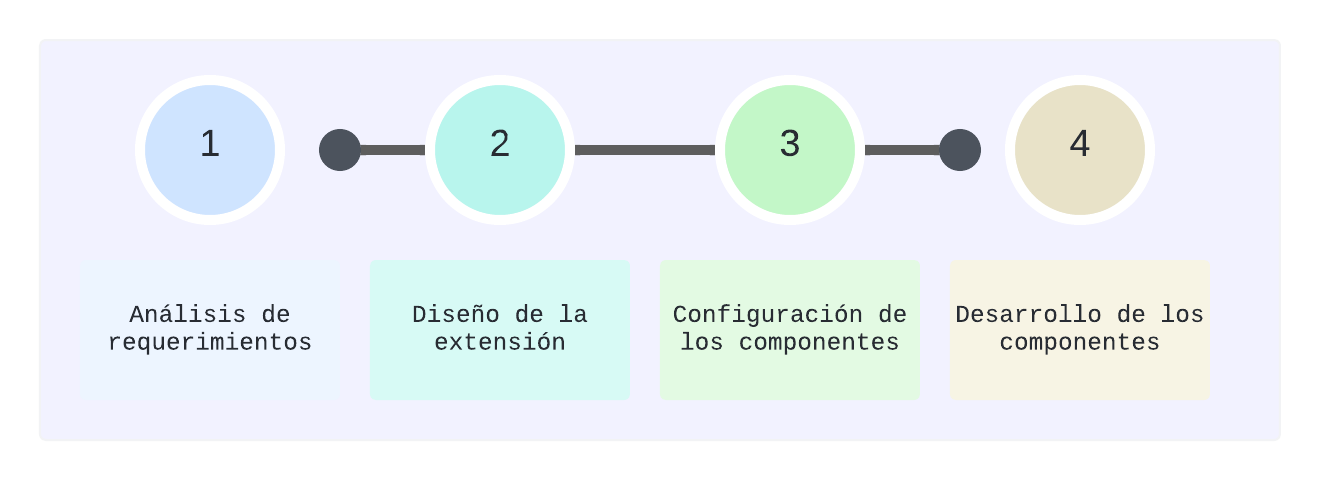
\includegraphics[width=310px]{cap3_fases_desarrollo.png}
	\caption{Fases de Desarrollo.}
	\label{fig:cap3_fases_desarrollo}
\end{figure}


\subsection{Fase 1: Análisis de requerimientos}

En esta fase, se han definido los requisitos funcionales y no funcionales que guiarán la extensión de la herramienta TDDT4IoTS, asegurando que cumpla con las necesidades específicas de los ingenieros de software que utilizan el sistema para analizar descripciones de casos de uso en entornos IoT.

\subsubsection{Identificación de usuarios y casos de uso}

La extensión puede funcionar exitosamente con la manipulación de dos tipos de perfiles de usuario, el desarrollador (ingenieros de software) y un administrador. A continuación se describen cada uno de los perfiles y como utilizan la extensión mediante la herramienta TDDT4IoTS:

\begin{itemize}
	\item \textbf{Desarrollador:} Es el usuario encargado de ingresar los datos de entrada mediante las descripciones del sistema IoT a desarrollar en forma de casos de uso extendidos. Mediante la herramienta podra transformar estas descripciones en un diagramas de clases y poder validar la arquitectura previa del sistema IoT. Además, sera el encargado de seleccionar el modelo de OpenAI que crea conveniente a utilizar.
	
	\item \textbf{Administrador:} Tendrá la posibilidad de registrar los modelos base de OpenAI y tener el privilegio de entrenar modelos, claramente deberá tener conocimiento sobre los modelos base que permitan realizar un ajuste fino, debido a que la herramienta necesita estos modelos para poder realizar los debidos entrenamientos y se puedan utilizar los modelos entrenados en los desarrollos de los sistemas IoT ingresados en la herramienta. 
\end{itemize}

Los casos de uso que se describen a continuación son las interacciones directas entre los perfiles de usuarios y la extensión. Cada caso de uso corresponde a una funcionalidad clave que la extensión debe proporcionar a los usuarios.

\begin{itemize}
	\item \textbf{Crear/Editar casos de uso:} El desarrollador puede crear o editar descripciones detalladas de casos de uso para sistemas IoT, introduciendo los actores y componentes involucrados. El sistema valida y almacena esta información.
	
	\item \textbf{Generar automáticamente el diagrama de clases:} A partir de las descripciones ingresadas, la extensión genera automáticamente un diagrama de clases conceptual utilizando el modelo base \textit{GPT-3.5} de OpenAI, que luego es almacenado y presentado gráficamente.
	
	\item \textbf{Entrenar modelos:} El usuario administrador tendrá el privilegio de poder entrenar los modelos que se crean necesarios y aporten un mejor funcionamiento a la herramienta mediante la extensión. 
	
	\item \textbf{Editar diagrama de clases generado:} Una vez generado el diagrama de clases completamente, el desarrollador podrá modificar el diagrama según las necesidades que crea conveniente. Los cambios realizados se guardaran dentro de la herramienta para futuras revisiones. 
\end{itemize}

La figura \ref{fig:cap3_diagramacasodeuso} muestra el diagrama de casos de uso identificado para comprender mejor el funcionamiento de la extensión sobre la herramienta. Permite identificar los actores principales y los casos de uso previamente mencionados. 

\begin{figure}[H]  
	\centering
	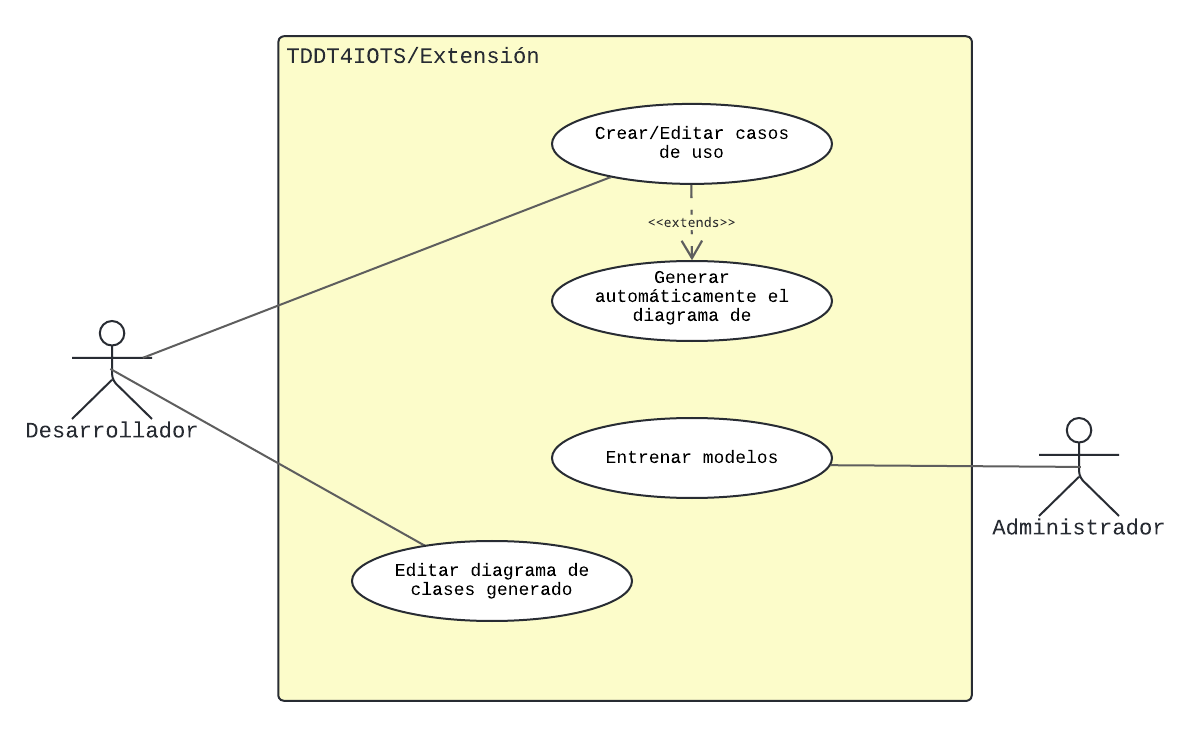
\includegraphics[width=350px]{diagramaCasosdeUso.png}
	\caption{Diagrama de casos de uso de la extensión.}
	\label{fig:cap3_diagramacasodeuso}
\end{figure}

\subsection{Fase 2: Diseño de la extensión}

En esta fase se explicará detalladamente el comportamiento de cada proceso necesario para que la extensión de la herramienta funcione correctamente. Se dedicó tiempo a analizar cuál sería la mejor forma de adaptar la nueva funcionalidad a la herramienta sin afectar los componentes existentes.

\subsubsection{Diseño de la arquitectura}

En esta subsección se explicara a detalle que tecnologías fueron necesarias implementar en cada capa y para que se utilizaron dichas tecnologías para lograr con el objetivo general y específicos del proyecto. 

\textbf{Capa del cliente}

\begin{itemize}
	\item \textbf{AngularJS:} Para mantener el correcto funcionamiento de la herramienta TDDT4IoTS, se decidió continuar utilizando este framework para generar las nuevas interfaces web. Esto permite que los usuarios perciban y usen la herramienta de la misma manera que lo hacían anteriormente.
\end{itemize}

\textbf{Capa de conexión}

\begin{itemize}
	\item \textbf{gRPC:} Este protocolo de comunicación facilita la integración interna de componentes en el servidor. Su objetivo es aprovechar las ventajas de diversas tecnologías y permitir que trabajen conjuntamente, asignando cargas de trabajo que pueden ser mejor ejecutadas por otras tecnologías.
	
	\item \textbf{HTTPS:} Es el protocolo estándar para el desarrollo de aplicaciones web. Permite enviar y recibir datos entre un navegador web y el servidor, lo que es esencial para cumplir con los objetivos de cualquier proyecto implementado. En la extensión de la herramienta, permite realizar las peticiones necesarias al servidor y obtener respuestas que se mostrarán a los usuarios finales.
	
\end{itemize}

\textbf{Capa de negocio}

\begin{itemize}
	\item \textbf{Spring Framework:} Para procesar todas las peticiones de la extensión, se utilizó el framework Spring, que emplea Java como lenguaje de programación. Java es conocido por su robustez y su capacidad para manejar un alto volumen de solicitudes. Considerando la cantidad de peticiones que se recibirán cuando se utilice la extensión mediante la herramienta, se busca mantener una conexión estable y aprovechar todas las ventajas que ofrece Spring Framework. Este framework es ideal para este proceso debido a su capacidad para manejar concurrencia, su soporte para transacciones, y su eficiente gestión de recursos. Además, Spring Framework permite ofrecer respuestas rápidas a las peticiones, gracias a su alta capacidad de procesamiento de datos y a su arquitectura modular, que facilita el mantenimiento y la escalabilidad de la aplicación.
	
	\item \textbf{NodeJs:} La herramienta cuenta con un intérprete que analiza la redacción de los casos de uso creados mediante la misma. Este intérprete, denominado ArmadilloJs, fue desarrollado como una librería JavaScript. Para generar los archivos necesarios para el entrenamiento de los modelos de OpenAI, surgió la necesidad de migrar la librería a un servicio web. Dado que la librería fue programada en JavaScript, se decidió implementar el servicio web con Node.js. Esta elección permite utilizar el intérprete de forma interna a través de los microservicios proporcionados por Spring Framework, aprovechando la compatibilidad y eficiencia de Node.js para manejar solicitudes asíncronas y el robusto manejo de transacciones y recursos de Spring Framework.
	
	\item \textbf{Python:} Como parte de la extension, se hace uso de la API de OpenAI. Python se destaca como uno de los lenguajes más utilizados en tecnologías de inteligencia artificial debido a su simplicidad, versatilidad y una amplia gama de bibliotecas especializadas. Aprovechando la existencia de una biblioteca de OpenAI para Python, se implementó la comunicación con OpenAI para mantener una interacción más fluida y bien desarrollada. Además, Python ofrece ventajas significativas en el desarrollo de aplicaciones de IA, como una sintaxis clara y legible, una gran comunidad de desarrolladores y soporte extensivo para frameworks y herramientas de aprendizaje automático y procesamiento de datos. Estas características hacen de Python la elección ideal para integrar OpenAI y aprovechar al máximo sus capacidades de IA en la herramienta.
	
\end{itemize}

\textbf{Capa de la nube}

\begin{itemize}
	\item \textbf{OpenAI:} La comunicación con la API de OpenAI permite utilizar los recursos almacenados en sus servidores. Esto da una ventaja de no utilizar recursos locales para implementar modelos de inteligencia artificial desde cero. También aprovechando los recursos de OpenAI se almacenan los datos entrenados por cada cuenta de usuario que este registrada en sus servicios. Cabe recalcar que también se almacena ciertos datos de forma local. 
\end{itemize}

\textbf{Capa de datos}

\begin{itemize}
	\item \textbf{PostgreSQL:} La comunicación con la API de OpenAI permite utilizar los recursos alojados en sus servidores, lo cual ofrece la ventaja de no necesitar recursos locales para implementar modelos de inteligencia artificial desde cero. Al aprovechar los recursos de OpenAI, los datos entrenados se almacenan por cuenta de usuario registrada en sus servicios. Además, es importante destacar que algunos datos también se almacenan localmente para mejorar la eficiencia y disponibilidad. Esta combinación de almacenamiento en la nube y local asegura un rendimiento óptimo y una gestión eficiente de los datos.
\end{itemize}

\subsubsection{Diseño de los componentes creados}

En la figura \ref{fig:cap3_integracion_componentes} se puede visualizar la comunicación entre todos los componentes que controlan el correcto funcionamiento de la extensión. El funcionamiento de los componentes es del a siguiente manera:

\begin{enumerate}
	\item \textbf{db-repository-tddt4iots:} Contiene todos los objetos necesarios para acceder a los datos de forma óptima.
	\item \textbf{ms-core-tddt4iots:} Mantiene separados los recursos reutilizables por toda la extensión, además de contener los DTO necesarios para las peticiones entre el cliente y el servidor.
	\item \textbf{ms-core-tddt4iots-openai:} Es el componente principal del proyecto, consumiendo los recursos de los componentes mencionados anteriormente, utilizados como dependencias mediante Maven.
	\item \textbf{ms\_core\_tddt4iots\_py:} Establece la comunicación con OpenAI y configura lo necesario para realizar entrenamientos e implementar los modelos.
	\item \textbf{armadillo-api:} API RestFul que interpreta casos de uso redactados en lenguaje de símbolos para obtener texto en lenguaje natural y crear archivos de entrenamiento.
\end{enumerate}

\begin{figure}[H]  
	\centering
	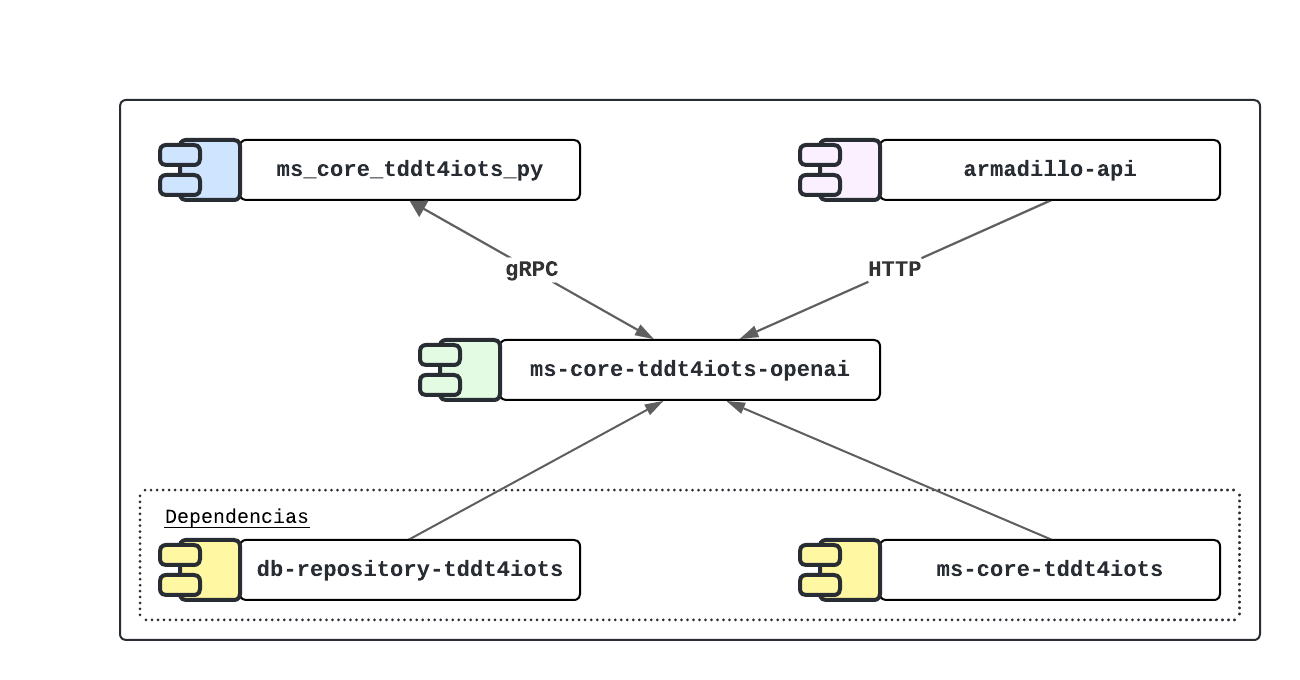
\includegraphics[width=\textwidth]{cap3_integracion_componentes.png}
	\caption{Componentes de la extensión.}
	\label{fig:cap3_integracion_componentes}
\end{figure}

\textbf{Modelos de IA}

OpenAI ofrece una variedad de modelos que pueden ser utilizados mediante el ajuste fino. Esta técnica permite entrenar modelos para especializarlos en tareas específicas, adaptándolos a las necesidades particulares del proyecto en el que se esté trabajando. Se llegó a la conclusión de registrar los posibles modelos base dentro de la herramienta, lo que permite seleccionar el modelo base adecuado para iniciar un nuevo entrenamiento y ponerlo a disposición de todos los usuarios.

Además, el proceso de ajuste fino no solo optimiza la precisión del modelo, sino que también mejora su eficiencia en la tarea específica, reduciendo el tiempo y los recursos necesarios para obtener resultados precisos. De esta manera, OpenAI asegura que sus usuarios puedan aprovechar al máximo las capacidades avanzadas de sus modelos de inteligencia artificial, facilitando la implementación de soluciones innovadoras y efectivas en diversos ámbitos.

\textbf{Entrenamiento de modelos}

El ajuste fino permitió entrenar modelos existentes para cumplir con los requisitos funcionales del proyecto. Cada entrenamiento quedará registrado dentro de la herramienta, permitiendo llevar un historial detallado de todos los entrenamientos realizados a los modelos seleccionados. Esta tarea es llevada a cabo por los usuarios interesados en entrenar modelos. Para entrenar modelos, se debe seguir una serie de pasos que se han tratado de automatizar por completo. Es necesario contar con una secret key de OpenAI para poder entrenar estos modelos. Además, se necesita un conjunto de datos que serán enviados al modelo mediante el ajuste fino y esperar los resultados del entrenamiento.

El archivo debe contener las posibles peticiones y respuestas que el modelo debe procesar cuando sea utilizado por otros usuarios mediante la herramienta. Este archivo actúa como una guía de comportamiento, asegurando que el modelo responda adecuadamente a diferentes escenarios. Además, es crucial que los datos estén bien estructurados y sean representativos de los casos de uso reales para garantizar la eficacia del entrenamiento. De esta manera, se optimiza el rendimiento del modelo y se mejora la precisión de sus respuestas, facilitando su integración y uso en aplicaciones prácticas.

\textbf{Uso de modelos}

Teniendo algunos modelos entrenados, se puede hacer uso de ellos para interpretar las descripciones de los casos de uso redactados en lenguaje natural. El usuario interesado en el entrenamiento realizado por otro usuario podrá seleccionarlo desde el historial de entrenamiento. Para llevar a cabo este proceso, también se debe contar con una secret key para poder acceder al modelo entrenado. Debido a que OpenAI solo permite acceder al modelo entrenado con la misma secret key con la que fue entrenado, se implementó la funcionalidad de compartir la secret key del usuario que entrenó el modelo para facilitar el acceso compartido.

\subsection{Fase 3: Configuración de los componentes}

En esta fase se detallan los componentes que fueron configurados para abarcar la funcionalidad completa de la extensión. Cada componente está diseñado para cumplir con una funcionalidad específica, asegurando que el sistema no solo cumpla con los requisitos actuales, sino que también sea escalable y mantenible a lo largo del tiempo. Se han tomado en cuenta prácticas de diseño modular y principios de ingeniería de software que permiten una fácil actualización y expansión de la herramienta, facilitando así su adaptación a futuras necesidades y mejoras tecnológicas.

\begin{itemize}
	\item \textbf{db-repository-tddt4iots: } Para mantener la conexión a la base de datos del proyecto, se configuró este componente como una dependencia del proyecto principal. El objetivo de este componente es centralizar todas las operaciones relacionadas con el acceso a datos, incluyendo el mapeo de entidades de la base de datos a clases Java, la ejecución de consultas SQL, y otras tareas de manejo de datos. Esta configuración permite una gestión más eficiente y organizada de las interacciones con la base de datos, asegurando un acceso a datos consistente y fiable.
	
	\item \textbf{ms-core-tddt4iots: } Este componente se encargará de contener todos los DTO necesarios para realizar las peticiones y respuestas, tanto del cliente al servidor como del servidor a la base de datos. Además, incluirá métodos utilitarios que podrán ser utilizados por otros componentes o proyectos generales, facilitando la reutilización de código y mejorando la eficiencia del desarrollo.
	
	\item \textbf{ms-core-tddt4iots-openai} Este componente constituye el proyecto principal y utiliza como dependencias los demás proyectos mencionados anteriormente. En este proyecto se configurarán todos los microservicios que se liberarán y que podrán ser consumidos por la extensión, asegurando así una integración fluida y coherente. Además, este proyecto se encarga de configurar los parámetros necesarios para acceder a la base de datos, manteniendo los objetos de datos aislados en sus respectivas dependencias. Esta separación de responsabilidades no solo mejora la organización del código, sino que también facilita el mantenimiento y la escalabilidad del sistema. Al centralizar la configuración de los microservicios y las conexiones a la base de datos, este componente principal actúa como el núcleo del sistema, permitiendo una gestión eficiente de las interacciones entre los diferentes módulos y garantizando que todas las partes del proyecto funcionen de manera integrada y eficiente. 
	
	\item \textbf{ms\_core\_tddt4iots\_py: } Para implementar el uso del lenguaje de programación Python, se configuró este proyecto como un servidor gRPC. Este componente facilita la comunicación eficiente y rápida con la API de OpenAI mediante las librerías correspondientes, permitiendo tanto el entrenamiento como el uso de los modelos existentes. Dentro de este proyecto, se gestionan todas las interacciones con OpenAI, asegurando que las solicitudes y respuestas sean manejadas de manera óptima. La configuración del servidor gRPC permite una comunicación robusta y de baja latencia entre los diferentes servicios y el backend de OpenAI, lo que es crucial para operaciones que requieren procesamiento en tiempo real. Además, este proyecto no solo se limita a gestionar el entrenamiento de los modelos, sino que también supervisa su implementación y actualización continua. Al utilizar gRPC, se garantiza que las conexiones sean seguras y eficientes, facilitando el desarrollo y la integración de nuevas funcionalidades basadas en IA.
	
	\item \textbf{armadillo-api: } La herramienta originalmente incluía un intérprete de descripciones de casos de uso redactadas en un lenguaje de símbolos. Este componente se configuró como un servicio web, permitiendo su utilización a través de una API REST que integra la biblioteca de JavaScript correspondiente. Esta configuración facilita el acceso y la interpretación de los casos de uso, asegurando que las descripciones sean procesadas de manera eficiente y precisa. Además, la implementación como servicio web permite una mayor flexibilidad y escalabilidad, permitiendo que otros sistemas y aplicaciones puedan interactuar con el intérprete de manera sencilla y consistente.

\end{itemize}

\subsection{Fase 4: Desarrollo de los componentes}

En esta fase se detalla todo lo desarrollado dentro de cada componente. Durante el desarrollo de esta fase, se logró aclarar y abordar todos los requisitos funcionales mencionados en la documentación del proyecto. A continuación, se describirán los paquetes implementados en cada componente y los pasos que se definieron para llevar a cabo la interpretacion de los casos de uso redactados en lenguaje natural para asegurar el funcionamiento completo de la extensión en la herramienta y satisfacer las necesidades del usuario final.

\begin{itemize}
	\item \textbf{db-repository-tddt4iots: } Dentro de este componente se empezó con el desarrollo de todos los paquetes necesarios para estructurar todos los objetos que intervienen en el manejo de los datos. 
	
	\begin{itemize}
		\item \textit{config:} configuración de los repositorios y transacciones JPA para la extensión de la herramienta.
		
		\item \textit{entity:} entidades que mapean las tablas de la base de datos.
		
		\item \textit{repository: } contiene todas las sentencias \texttt{SQL} que permitirán obtener los datos para las entidades.
		
		\item \textit{impl: } implementaciones de las interfaces del paquete \textit{service} para liberar los métodos existentes al proyecto que esté utilizando este componente como dependencia (ver figura \ref{fig:cap3_comp_db_pack}).
	\end{itemize}

	
	\begin{figure}[H]
		\centering
		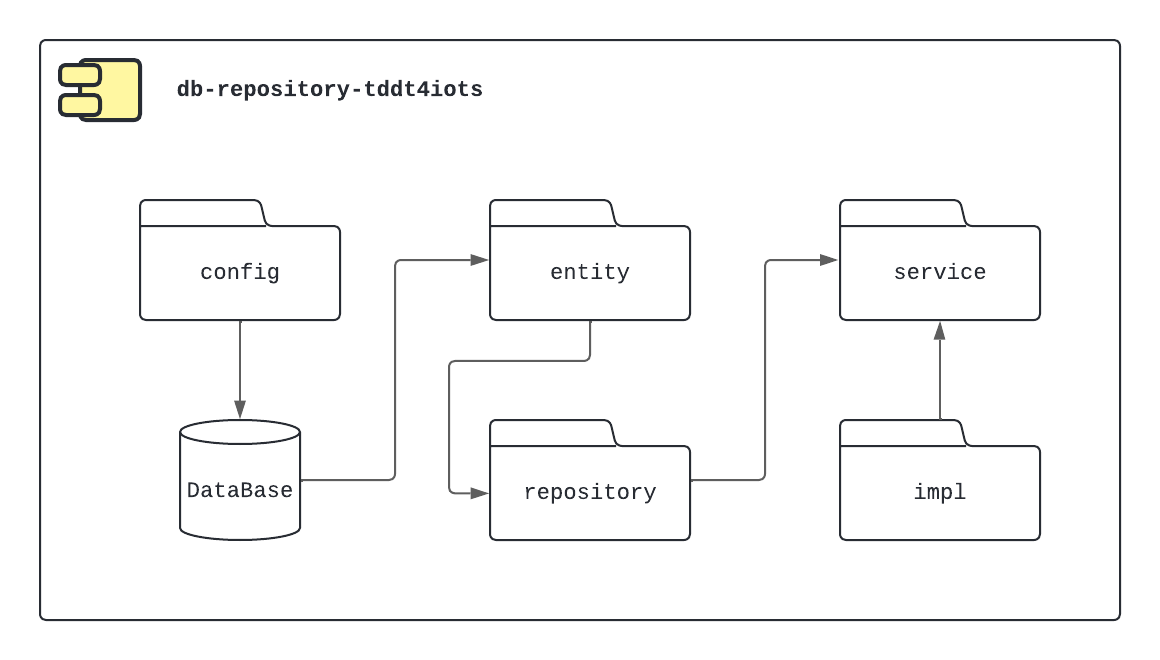
\includegraphics[width=\textwidth]{cap3_comp_db_pack.png}
		\caption{Paquetes desarrollados dentro del componente db-repository-tddt4iots.}
		\label{fig:cap3_comp_db_pack}
	\end{figure}
	
	\item \textbf{ms-core-tddt4iots: } Se estructura en varios paquetes, cada uno con objetivos específicos: 
	
	\begin{itemize}
		\item \textit{config: } configuración necesaria para la comunicación gRPC y puede ser escalable para desarrollar otras clases que permitan la conexión con otros tipos de protocolo
		\item \textit{cons: } almacena constantes utilizadas en todo el proyecto
		\item \textit{util: } contiene utilidades y funciones auxiliares reutilizables
		\item \textit{proto: } incluye los archivos \texttt{.proto} que definen los métodos y mensajes gRPC para la interacción entre componentes
		\item \textit{dto: } alberga los \textit{Data Transfer Objects} (DTO).
		\item \textit{grpc\_service: } contiene las implementaciones de los servicios gRPC definidos en los archivos .proto, asegurando una integración eficiente y consistente en todo el proyecto (ver figura \ref{fig:cap3_comp_core_pack}).
	\end{itemize}

	
	\begin{figure}[H]
		\centering
		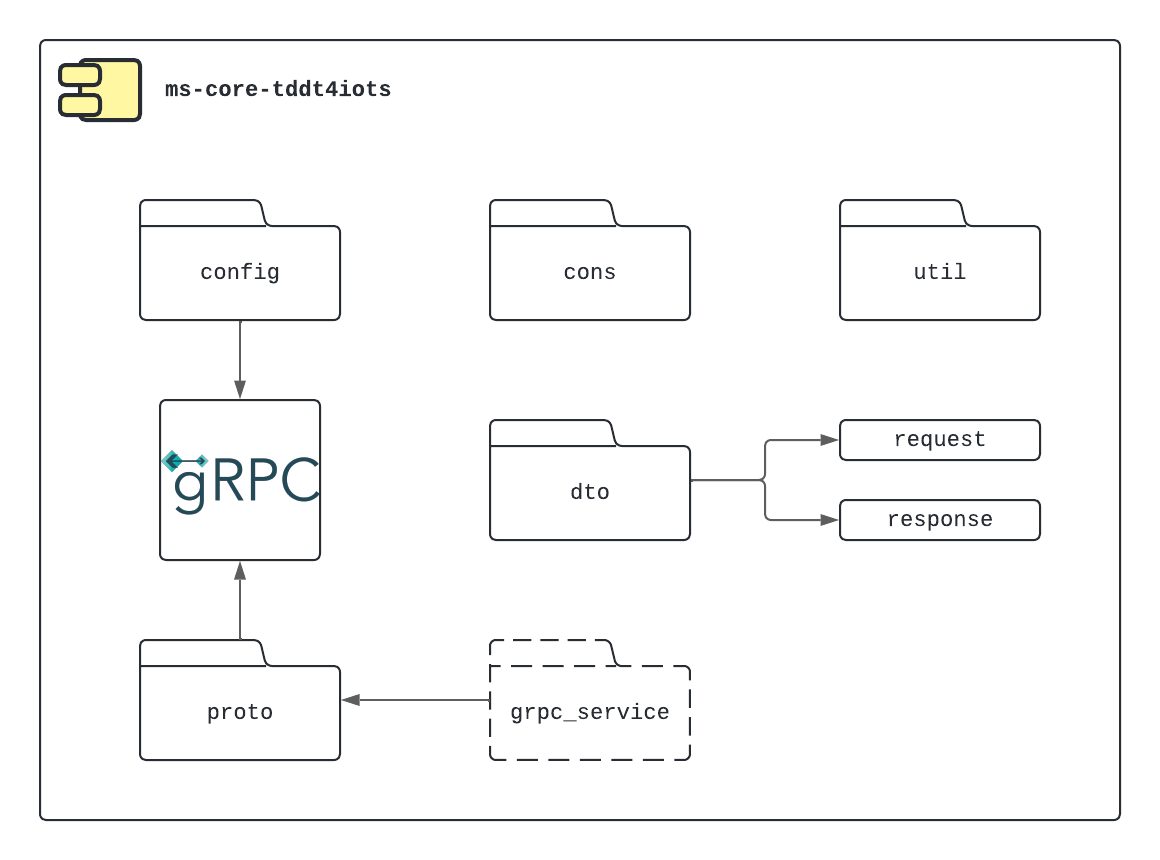
\includegraphics[width=\textwidth]{cap3_comp_core_pack.png}
		\caption{Paquetes desarrollados dentro del componente ms-core-tddt4iots.}
		\label{fig:cap3_comp_core_pack}
	\end{figure}
	
	\item \textbf{ms-core-tddt4iots-openai: } La figura \ref{fig:cap3_comp_core_openai_pack} muestra la estructura y como se comunican los paquetes dentro de este componente. A continuación se detalle el funcionamiento de cada paquete:
	
	\begin{itemize}
		\item \textit{config}: gestiona la configuración necesaria para el funcionamiento del proyecto, configura el uso de las propiedades declaradas en el archivo \texttt{application.properties} y también incluye la configuración del cliente \texttt{gRPC}.
		\item \textit{rest}: se encarga de las interfaces \texttt{REST}, permitiendo la interacción del proyecto a través de llamadas HTTP.
		\item \textit{communication}: alberga la lógica de comunicación tanto \texttt{gRPC} como \texttt{REST}, facilitando la interacción fluida entre los componentes internos y externos.
		\item \textit{bo}: define las clases de negocio y la lógica empresarial, encapsulando los procesos del sistema.
		\item \textit{impl}: contiene las implementaciones concretas de estas interfaces y servicios.
		\item \textit{grpc}: maneja las operaciones relacionadas con \texttt{gRPC}, asegurando una comunicación eficiente con el servidor de Python que utiliza la librería de OpenAI.
		\item \textit{mapper}: incluye los mapeadores necesarios para convertir entidades entre diferentes capas del sistema.
		\item \textit{datasource}: gestiona las fuentes de datos, configurando las conexiones a la base de datos y otros servicios de almacenamiento.
	\end{itemize}
	
	\begin{figure}[H]
		\centering
		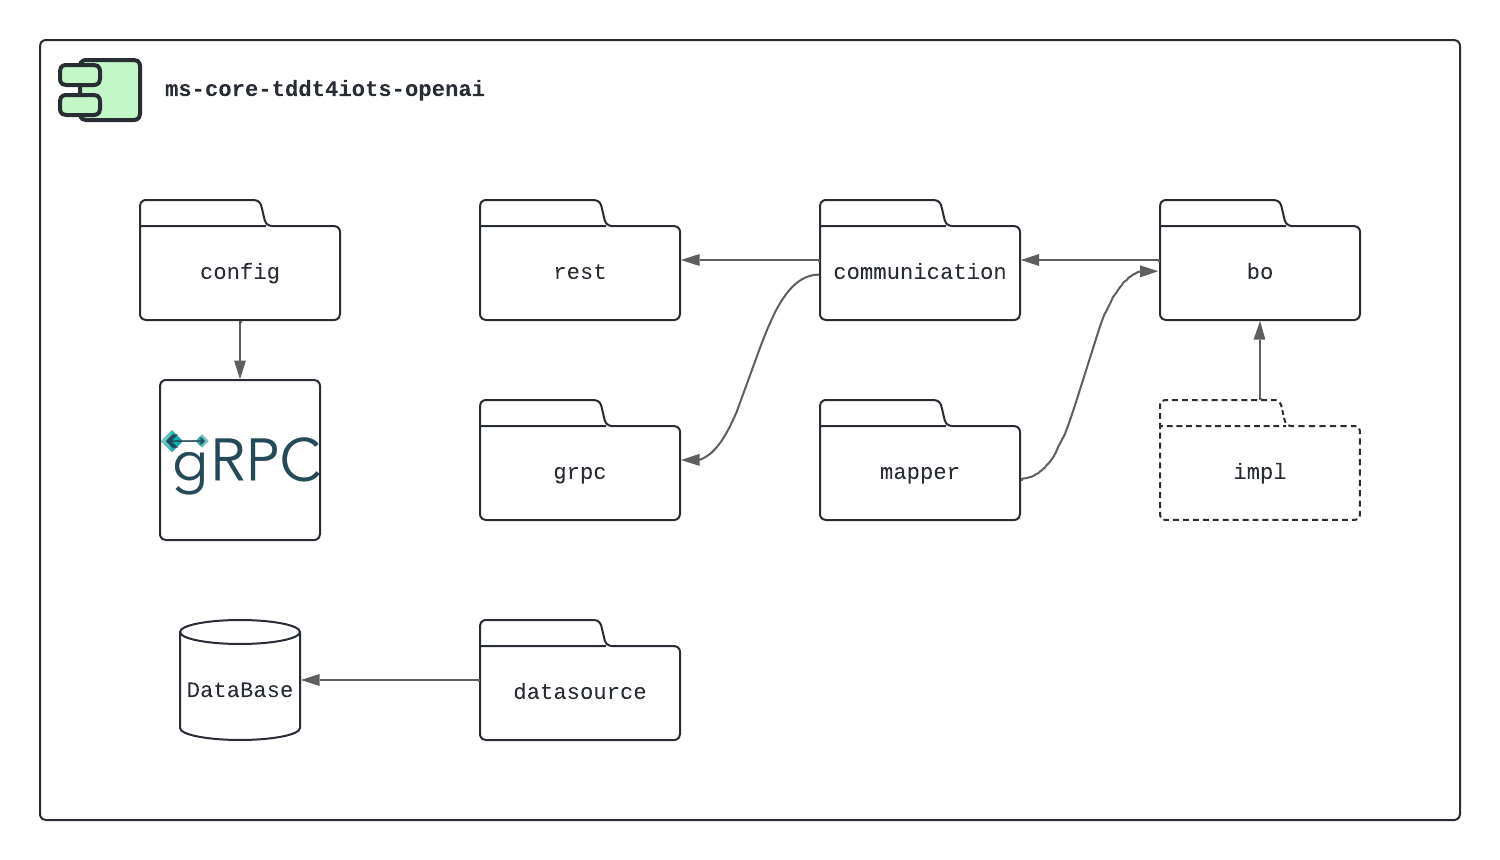
\includegraphics[width=300px]{cap3_comp_core_openai_pack.png}
		\caption{Paquetes desarrollados dentro del componente ms-core-tddt4iots-openai.}
		\label{fig:cap3_comp_core_openai_pack}
	\end{figure}
	
	Dentro de este componente se detallan los tres microservicios que realizan las tareas principales del proyecto:
	
	\begin{enumerate}
		\item Creación de los archivos en formato  \texttt{JSONL} que almacenarán los \texttt{prompt}, especificando los posibles mensajes de entrada y salida que el modelo debería devolver.
		\item Entrenamiento de el modelo, especificando los pasos que la extensión realizará de forma interna para llevar a cabo el entrenamiento de los modelos específicos almacenados localmente.
		\item 	Uso de un modelo entrenado, detallando cómo se recibirá la solicitud del cliente y cómo el modelo devolverá la respuesta esperada.
	\end{enumerate}
	
	En la figura \ref{fig:cap3_diagrama_secuencia_tarea1} se detalla el proceso analizado para la creación de los archivos \texttt{JSONL} y su almacenamiento, los cuales serán utilizados posteriormente en el entrenamiento de los modelos de OpenAI. 
	
		\begin{figure}[H]  
		\centering
		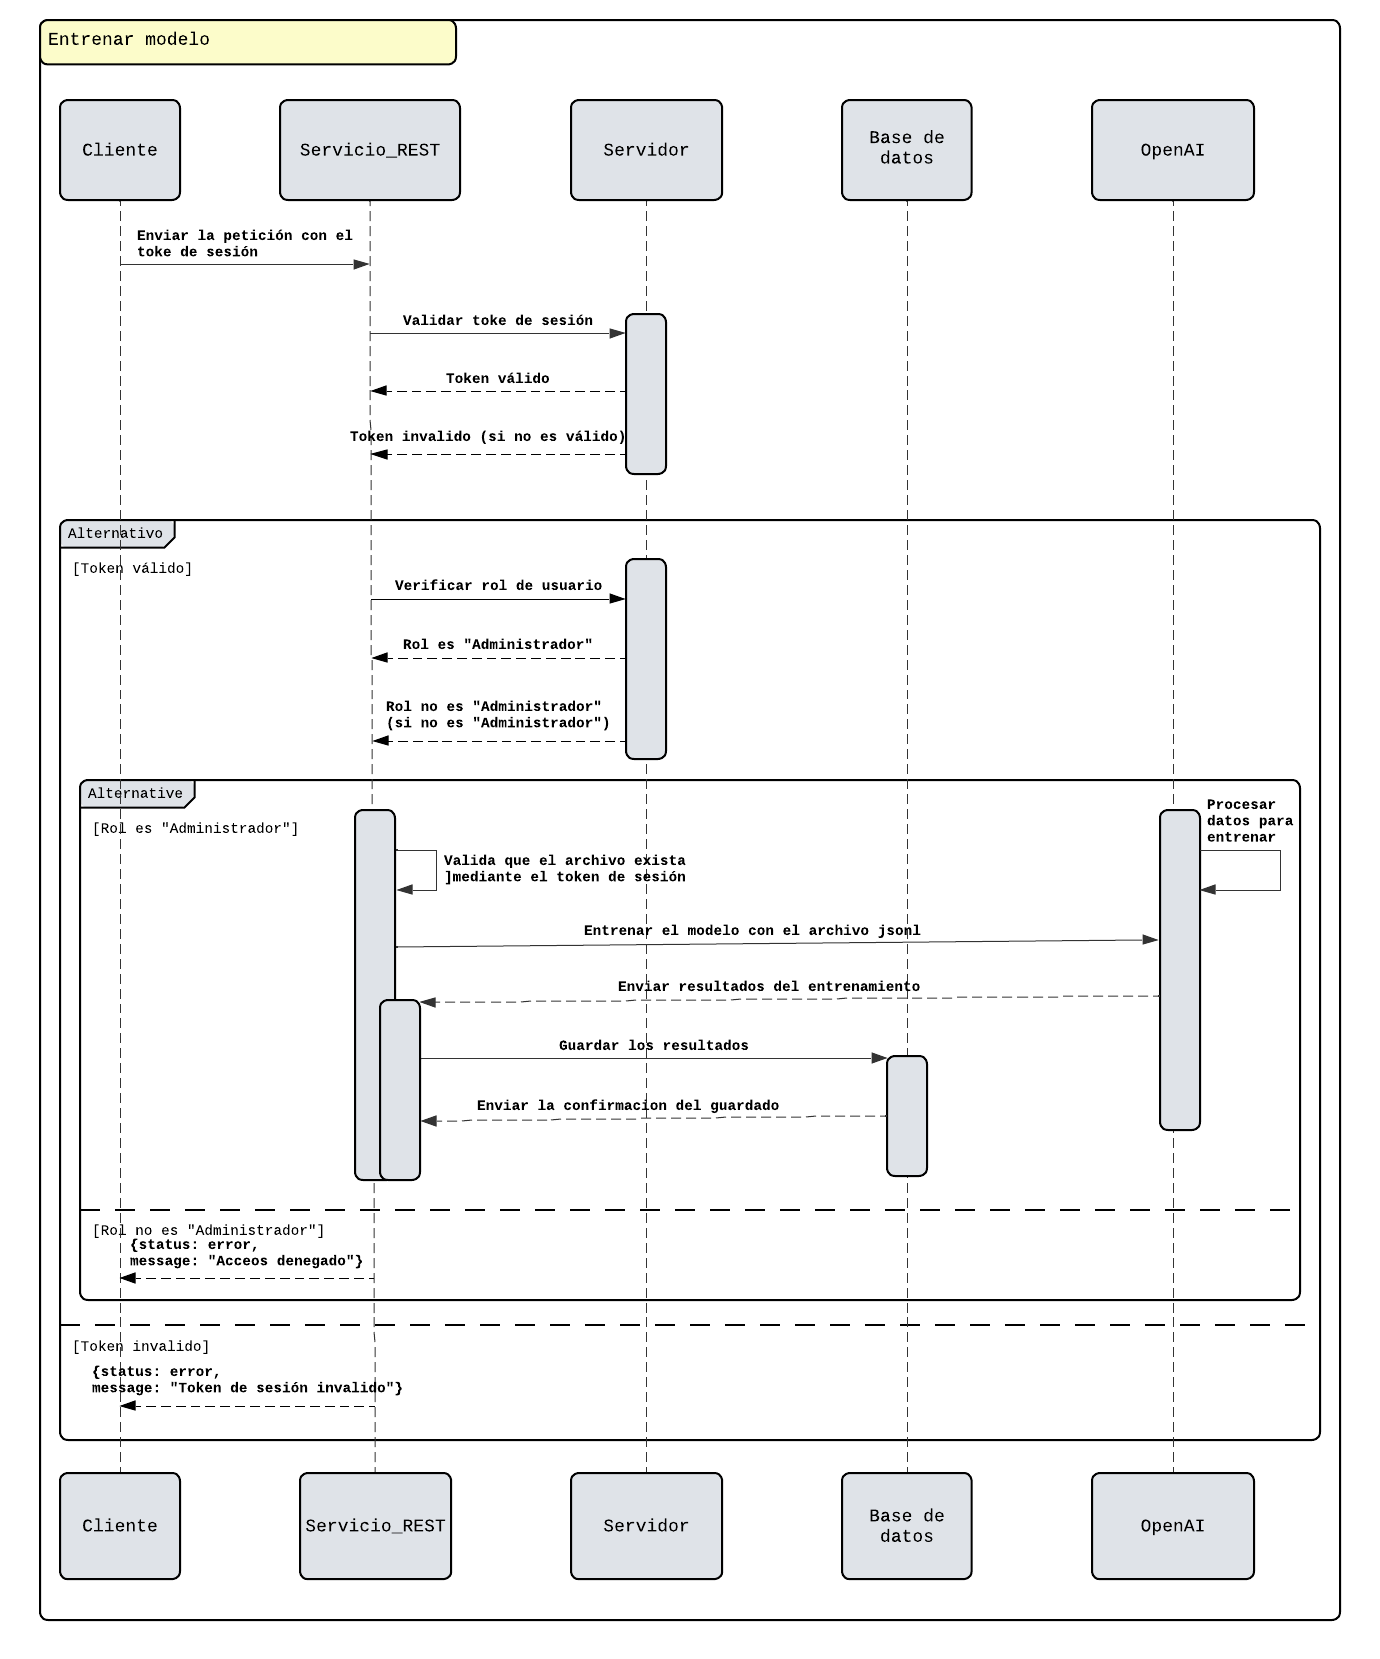
\includegraphics[width=310px]{cap3_diagrama_secuencia_tarea2.png}
		\caption{Diagrama de secuencia para explicar a detalle el proceso de entrenamiento del modelo mediante el archivo jsonl.}
		\label{fig:cap3_diagrama_secuencia_tarea2}
	\end{figure}	
	
	Este diagrama de secuencia ilustra cada paso necesario, desde la generación de los prompts hasta su estructuración en archivos \texttt{JSONL}, así como la ubicación específica donde estos archivos serán almacenados. el Cliente envía una petición con un token de sesión al Servicio REST, que verifica el token con el Servidor. Si el token es válido, el servidor procede a validar el rol del usuario (requiriendo el rol de ``Administrador"). Si el rol es correcto, el sistema valida la existencia del archivo para el entrenamiento y envía los datos a la API de OpenAI para procesar el modelo, almacenando luego los resultados en la Base de Datos. Aunque en la implementación real el Servicio REST y el Servidor podrían ser el mismo objeto, se han separado en el diagrama para detallar mejor las responsabilidades: el Servicio REST maneja la interacción inicial con el cliente, mientras que el Servidor gestiona la lógica interna de validación de roles y el procesamiento de solicitudes complejas, asegurando claridad en el flujo de validación y manejo de datos.
	
	La figura \ref{fig:cap3_diagrama_secuencia_tarea2} proporciona una visión clara y estructurada del flujo de acciones necesarias para el entrenamiento del modelo, asegurando que cada etapa del proceso se realice de manera correcta. Comenzando con el Cliente enviando una petición que incluye un token de sesión al Servicio REST. El Servicio REST valida el token consultando con el Servidor. Si el token es válido, el flujo continúa; de lo contrario, se devuelve un mensaje de error al cliente. En el caso de que el token sea válido, el Servidor verifica si el usuario tiene el rol de ``Administrador". Si el rol es correcto, el flujo avanza para validar la existencia del archivo para el entrenamiento del modelo. El Servidor luego procede a enviar el archivo a la API de OpenAI para entrenar el modelo, y los resultados obtenidos son almacenados en la Base de Datos. Finalmente, el servidor envía una confirmación al cliente una vez que los resultados se han guardado correctamente.
		
	Finalmente, la figura \ref{fig:cap3_diagrama_secuencia_tarea3} muestra cómo el Cliente envía una petición con un token de sesión y un texto en lenguaje natural al Servicio REST, que valida el token consultando al Servidor. Si el token es válido, el servidor verifica el rol del usuario (debe ser Administrador o Desarrollador) y, si es correcto, envía el texto a la API de OpenAI para que lo interprete. La API devuelve una respuesta en formato JSON, que es reenviada al cliente con un mensaje de éxito. Si el rol o el token no son válidos, se devuelve un mensaje de error. Aunque el Servicio REST y el Servidor podrían ser un único componente, se han separado en el diagrama para detallar mejor las responsabilidades: el Servicio REST maneja la autenticación y el Servidor gestiona la lógica de roles y el envío de la solicitud a OpenAI.
		
	\begin{figure}[H]  
		\centering
		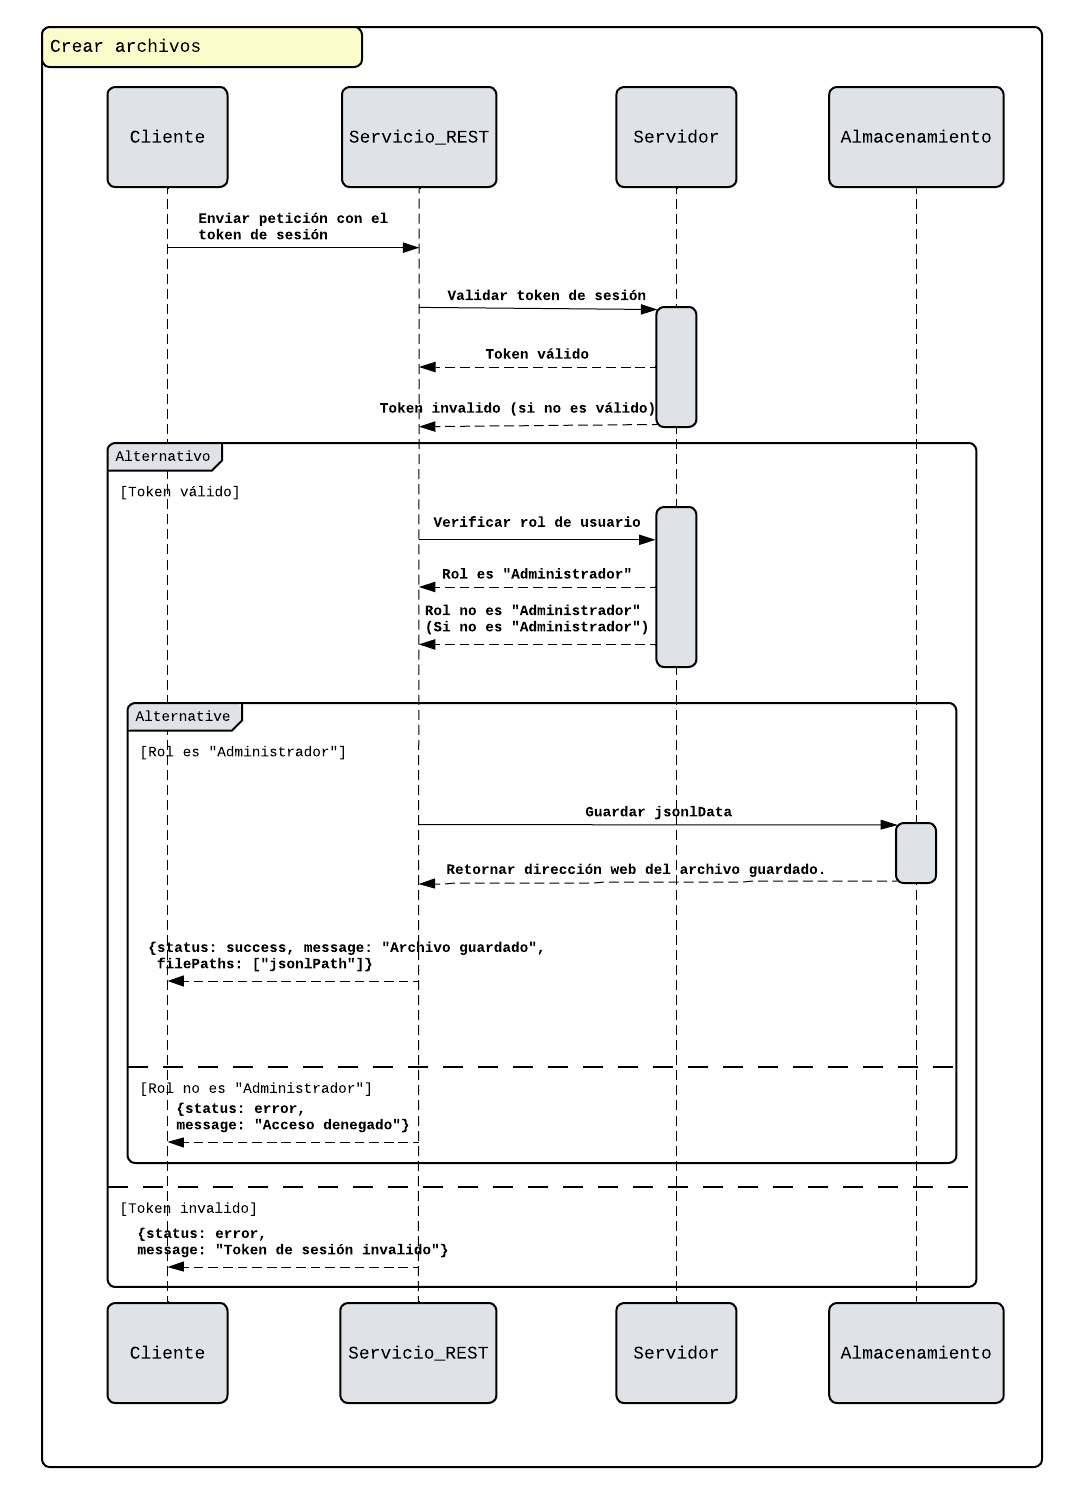
\includegraphics[width=\textwidth]{cap3_diagrama_secuencia_tarea1.png}
		\caption{Diagrama de secuencia para explicar a detalle el proceso de crear los archivos jsonl.}
		\label{fig:cap3_diagrama_secuencia_tarea1}
	\end{figure}	
	
	\begin{figure}[H]  
		\centering
		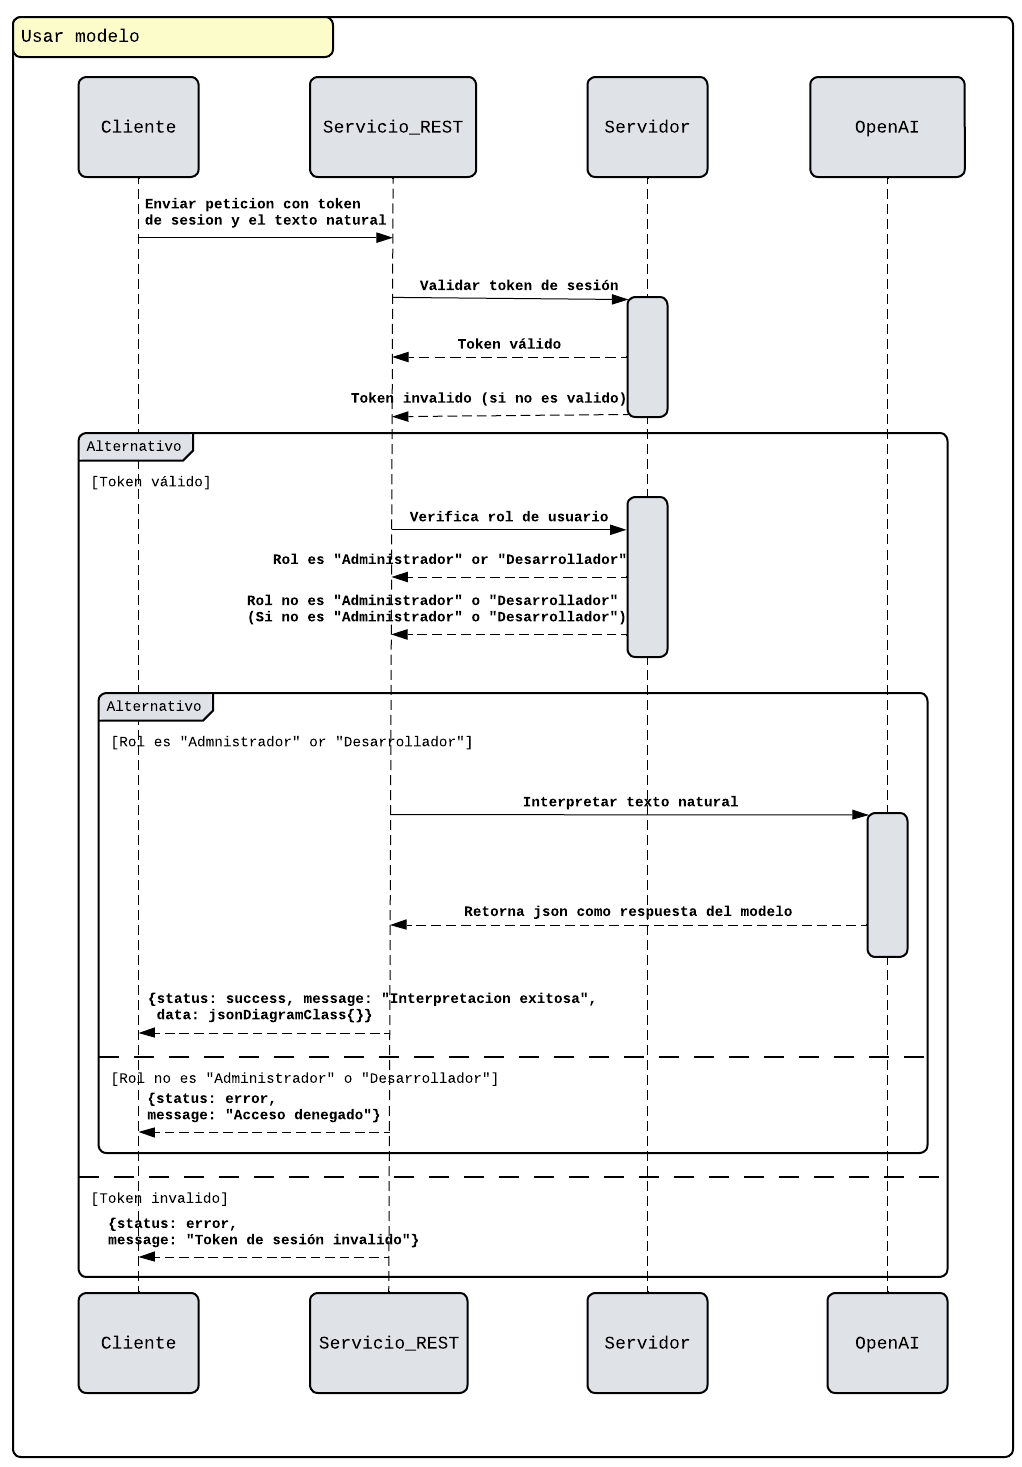
\includegraphics[width=\textwidth]{cap3_diagrama_secuencia_tarea3.png}
		\caption{Diagrama de secuencia para explicar a detalle el proceso de usar  el modelo.}
		\label{fig:cap3_diagrama_secuencia_tarea3}
	\end{figure}

	\newpage
	\item \textbf{ms\_core\_tddt4iots\_py: } En este componente se desarrolló el servidor gRPC para lograr la comunicación con el componente ms-core-tddt4iots-openai, con el objetivo de mantener los microservicios REST de Spring conectados con el cliente de AngularJS. Se implementaron dos métodos principales: uno para el entrenamiento del modelo y otro para su utilización, asegurando una integración eficiente y efectiva entre los distintos componentes del sistema (ver figura \ref{fig:cap3_comp_python_pack}).
	
	\begin{figure}[H]  
		\centering
		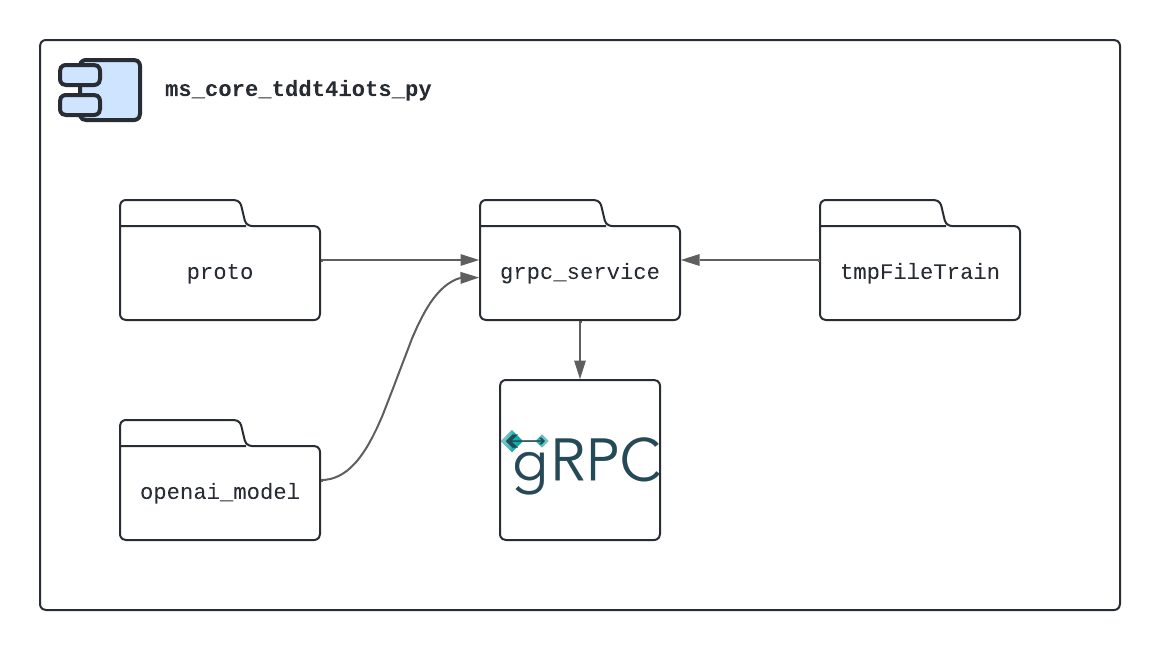
\includegraphics[width=10cm]{cap3_comp_python_pack.png}
		\caption{Paquetes desarrollados dentro del componente de python.}
		\label{fig:cap3_comp_python_pack}
	\end{figure}
		
	\begin{itemize}
		\item \textit{proto}: contiene los archivos \texttt{.proto} que definen las especificaciones de los servicios y mensajes \texttt{gRPC}, fundamentales para generar el código de comunicación.
		\item \textit{grpc\_service}: implementa estos servicios gRPC, facilitando la comunicación entre el servidor y otros componentes.
		\item \textit{tmpFileTrain}: es responsable de almacenar los archivos JSONL descargados, que son utilizados para el entrenamiento de los modelos.
		\item \textit{openai\_model}: alberga toda la lógica necesaria para conectarse y interactuar con la API de OpenAI, manejando las solicitudes y respuestas para integrar las funcionalidades de OpenAI en el proyecto.
	\end{itemize}
	
	
	En la figura \ref{fig:cap3_diagrama_flujo_proceso_a} se muestra el diagrama de flujo sobre el procedimiento seguido para el entrenamiento del modelo. El método recibe una solicitud con formato de cadena JSON con los parámetros necesarios, configura el cliente de OpenAI con una clave API, descarga el archivo JSONL desde la URL especificada, y lo guarda localmente

	\begin{figure}[H]  
		\centering
		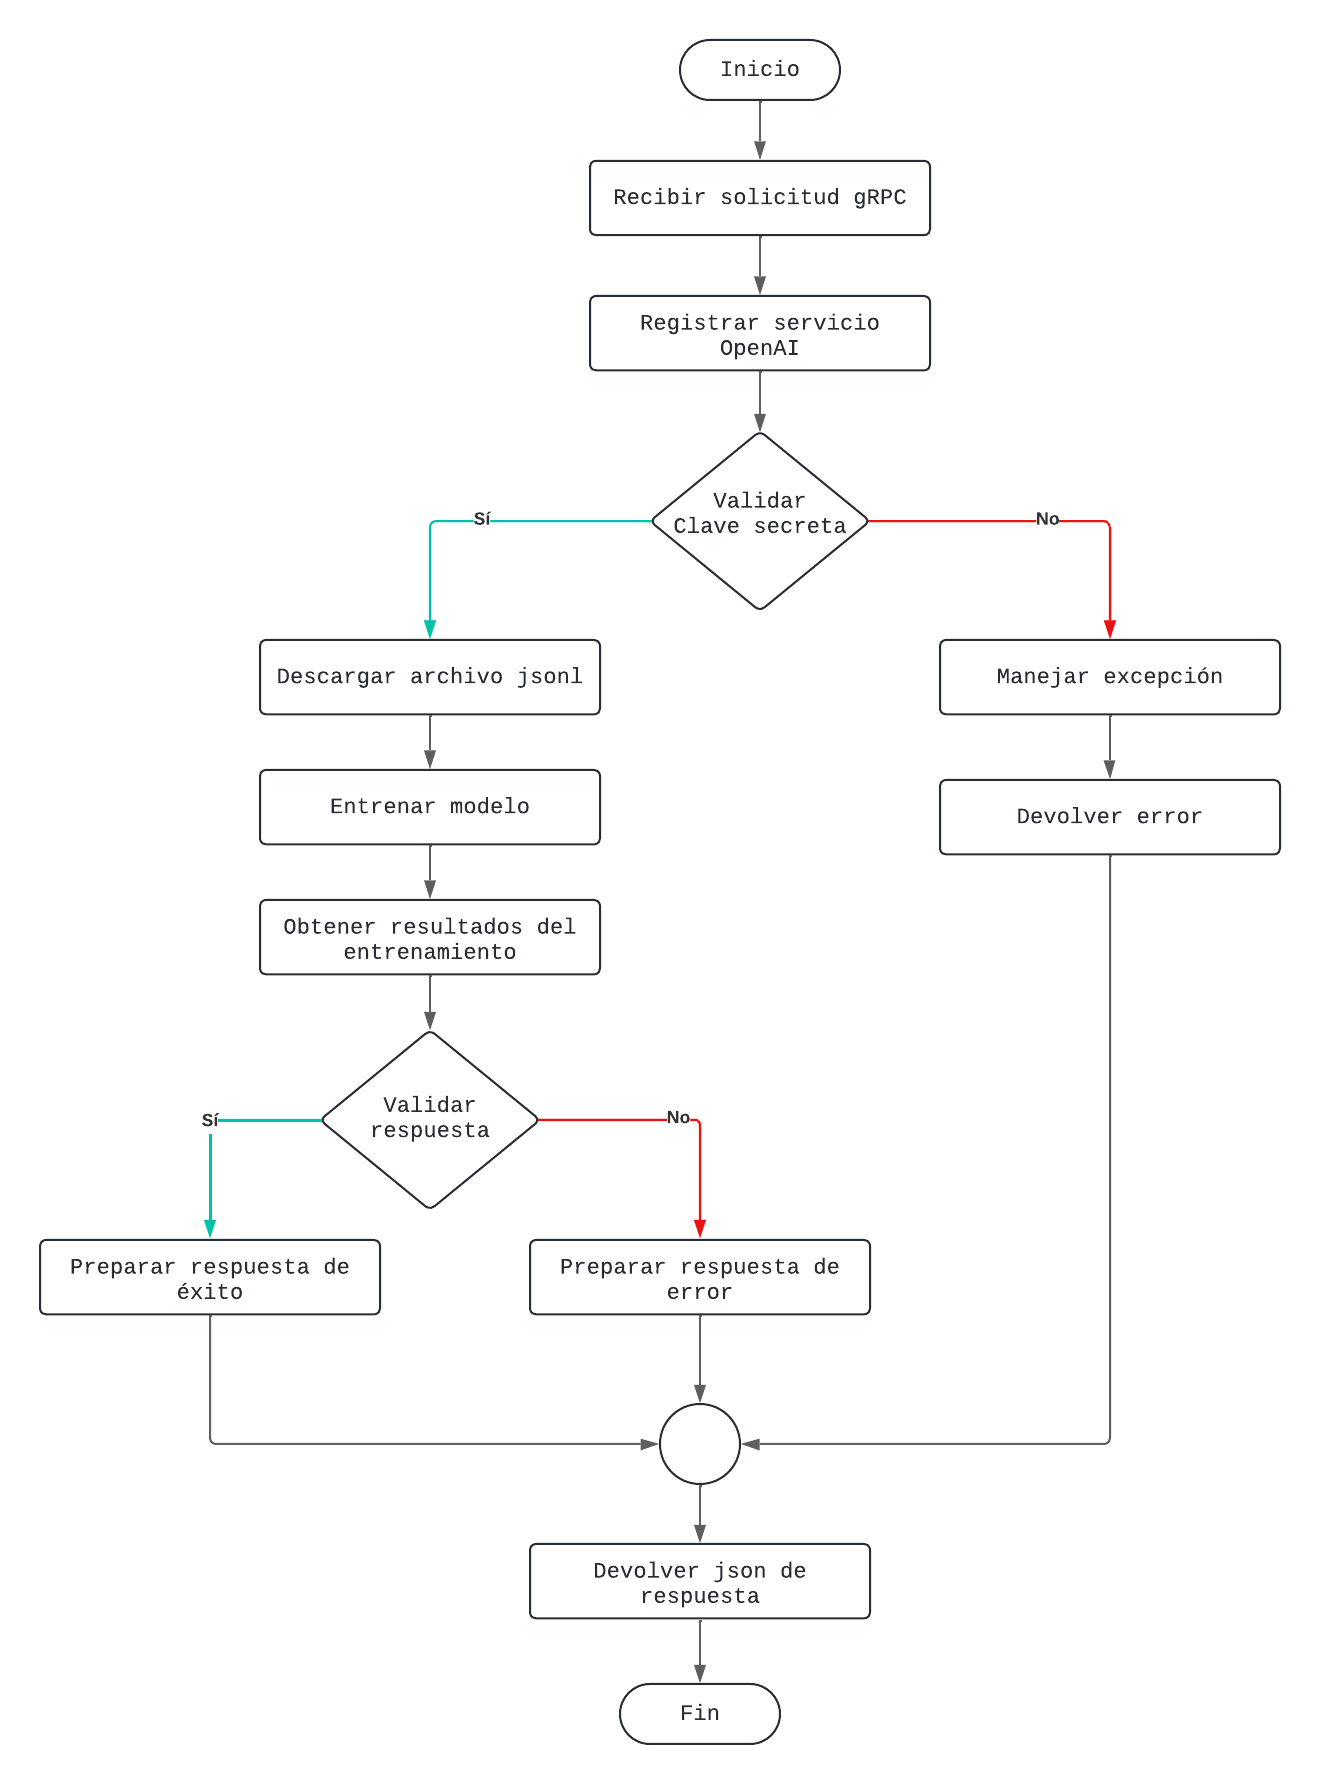
\includegraphics[width=\textwidth]{cap3_diagrama_flujo_proceso_a.png}
		\caption{Entrenamiento de los modelos de OpenAI.}
		\label{fig:cap3_diagrama_flujo_proceso_a}
	\end{figure}
	Luego, sube este archivo a OpenAI para iniciar el proceso de fine-tuning del modelo especificado. Si el proceso se realiza con éxito, devuelve un JSON indicando el estado del entrenamiento y los detalles del fine-tuning. En caso de error, retorna un mensaje de error.
	
	\begin{figure}[H]  
		\centering
		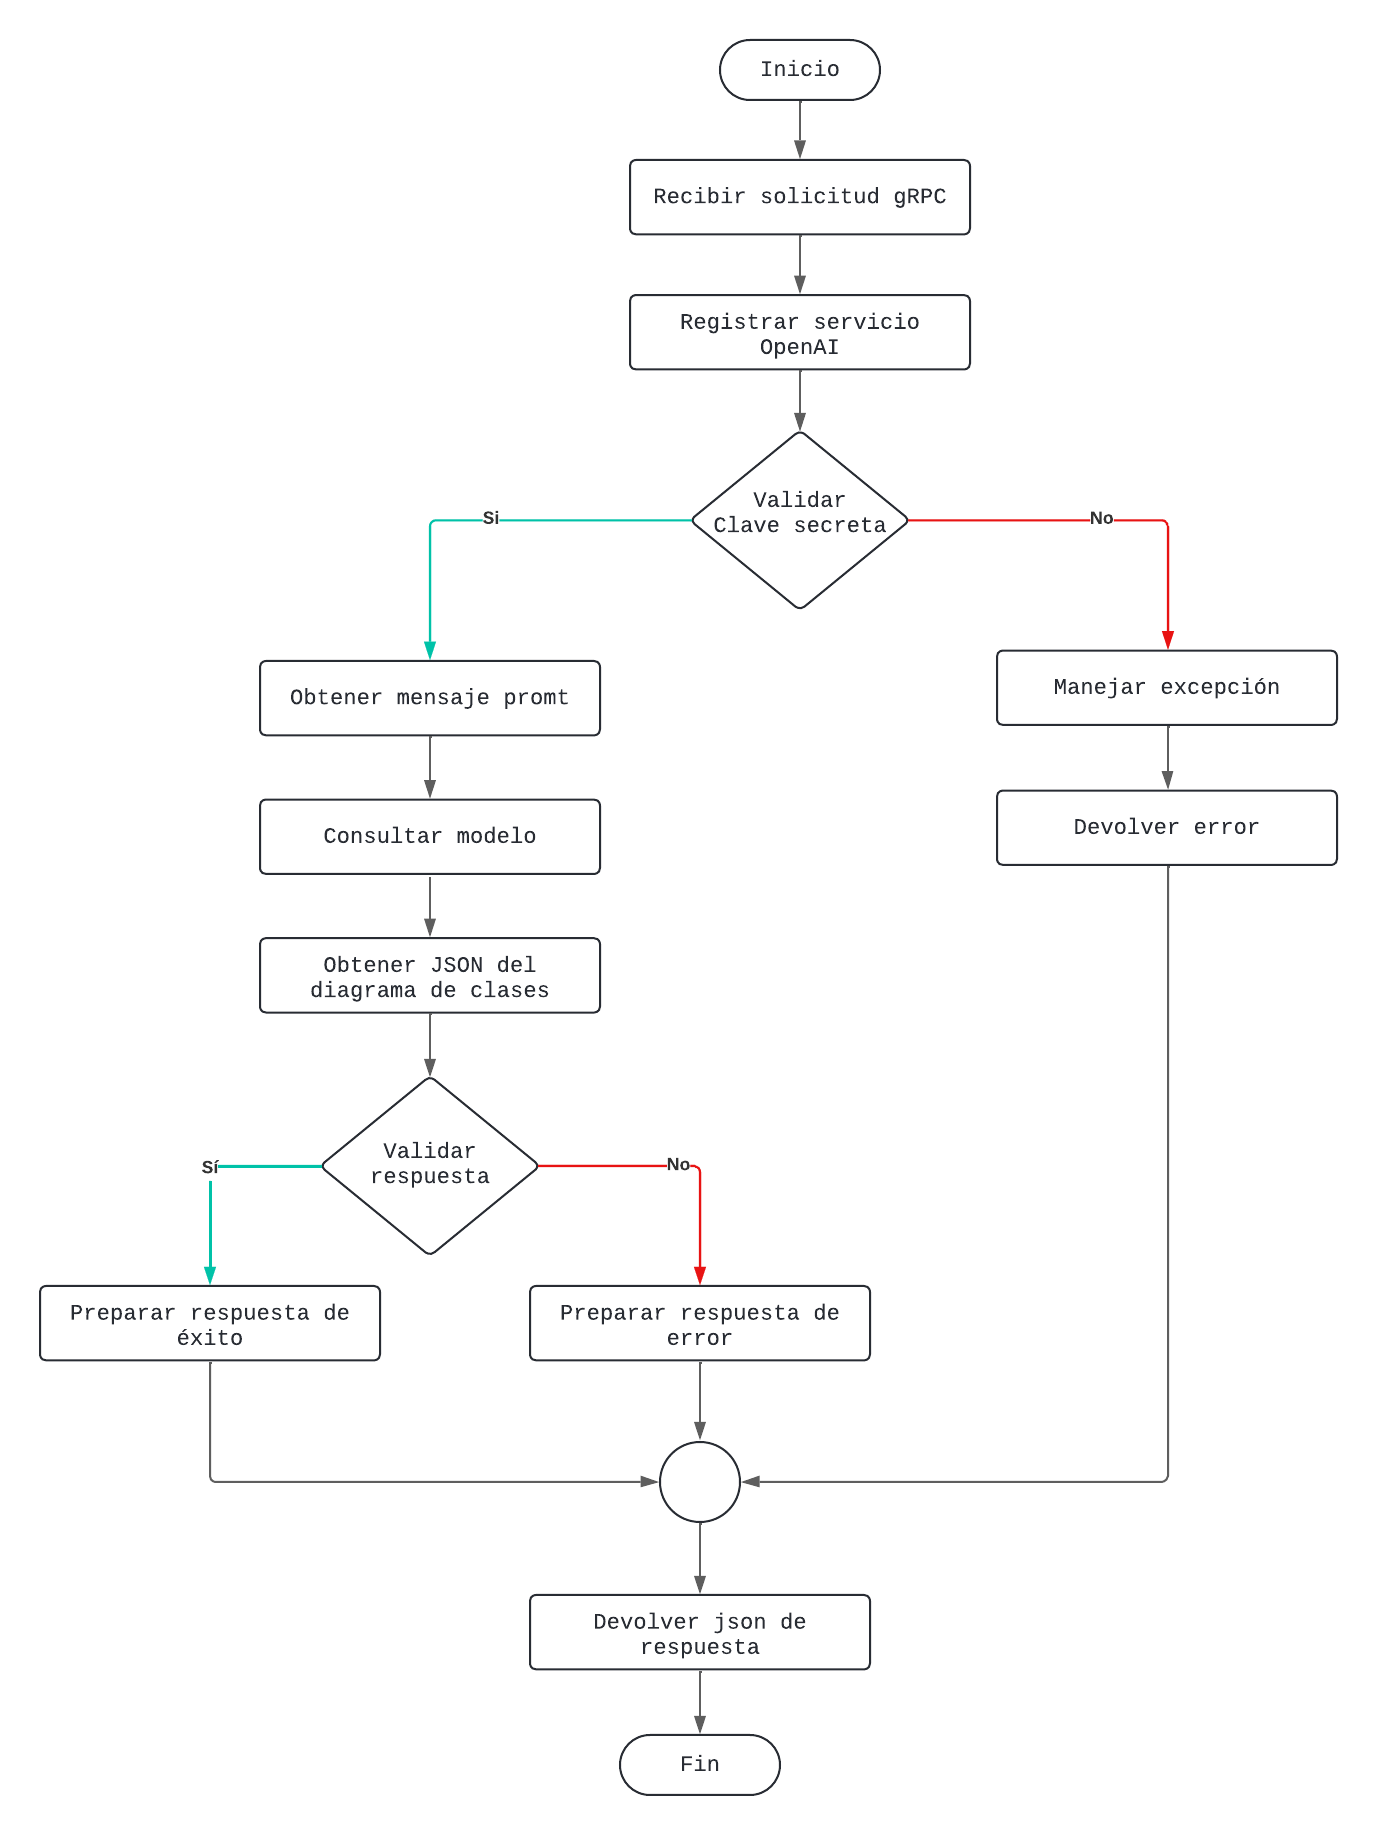
\includegraphics[width=\textwidth]{cap3_diagrama_flujo_proceso_b.png}
		\caption{Uso de los modelos entrenados por OpenAI.}
		\label{fig:cap3_diagrama_flujo_proceso_b}
	\end{figure}
	
	Para utilizar un modelo entrenado, es fundamental contar con un modelo base previamente entrenado con los datos extraídos de la herramienta. En la figura \ref{fig:cap3_diagrama_flujo_proceso_b} se muestra el proceso paso a paso que se sigue para garantizar el correcto funcionamiento de la extensión y su uso eficiente con la API de OpenAI. El proceso es muy similar al anterior con la deferencia que existe un paso denominado \texttt{Obtener mensaje promt}. Este paso contiene el texto redactado en lenguaje natural y ademas 1 mensaje en especifico detallando lo que debe realizar el modelo entrenado. 
	
	\item \textbf{armadillo-api: } En la herramienta actual, había un intérprete denominado ArmadilloJs que permitía convertir las descripciones de los casos de uso redactados en un conjunto de símbolos, los cuales identificaban los componentes para su diagrama de clases. Este intérprete estaba desarrollado como una biblioteca de JavaScript. Sin embargo, se ha planteado la necesidad de transformar esta biblioteca en un servicio web, para poder utilizar sus funciones internamente dentro del componente que entrena el modelo de inteligencia artificial. El objetivo de esta transformación es interpretar las descripciones de los casos de uso de los proyectos existentes y obtener el texto en lenguaje natural, con el fin de entrenar el modelo de inteligencia artificial de manera más eficaz (ver figura \ref{fig:cap3_comp_armadillo}). 
	
	\begin{figure}[H]  
		\centering
		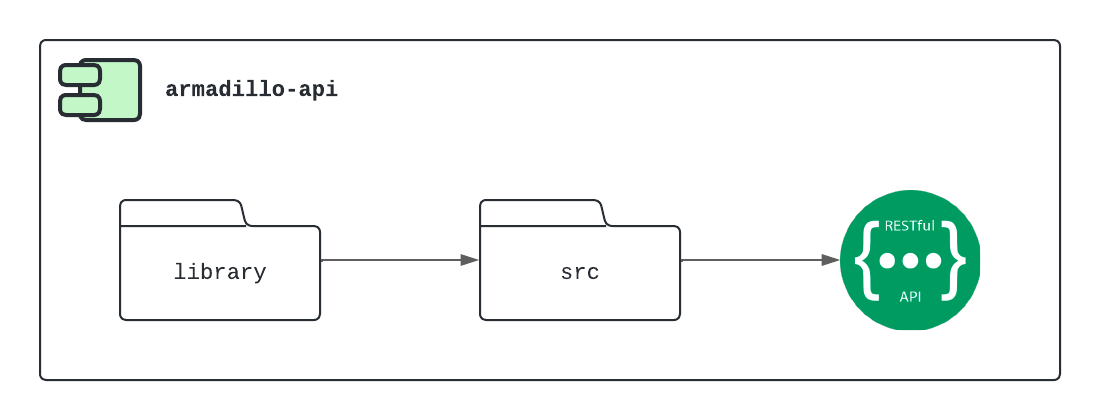
\includegraphics[width=\textwidth]{cap3_comp_armadillo.png}
		\caption{Estructura de los paquetes para el componente armadillo-api.}
		\label{fig:cap3_comp_armadillo}
	\end{figure}
	
\end{itemize}

\subsubsection{Herramientas de soporte al desarrollo de software}

Durante el desarrollo de nuestro proyecto, se utilizaron diversas herramientas de software proporcionadas por JetBrains (\url{https://www.jetbrains.com}) para maximizar la eficiencia y productividad. JetBrains ofrece un conjunto robusto de entornos de desarrollo integrado (IDE) que se adaptan a diversas necesidades y lenguajes de programación. El uso de estas herramientas avanzadas nos permitió abordar diversas fases del desarrollo con mayor eficiencia y precisión. Las herramientas utilizadas y su aportación al desarrollo del software realizado se describen a continuación.

\textbf{IntelliJ IDEA}

Para el desarrollo en Java, utilizamos \textbf{\textit{IntelliJ IDEA 2024.1.4}}, que proporcionó un entorno robusto y eficiente. Este IDE fue fundamental para la integración de Spring Framework y la gestión de microservicios, permitiéndonos escribir, probar y depurar código de manera efectiva. Las características avanzadas de IntelliJ, como la autocompletación inteligente, el análisis de código en tiempo real y las herramientas de refactorización, mejoraron significativamente nuestra productividad y calidad del código.

\textbf{WebStorm}

En el desarrollo de interfaces web, \textbf{\textit{WebStorm 2023.3.1}} fue la herramienta elegida por su capacidad para manejar tecnologías modernas como AngularJS. WebStorm facilitó la creación de interfaces web responsivas y dinámicas, proporcionando un entorno de desarrollo con soporte completo para JavaScript, TypeScript, HTML y CSS. Las capacidades de depuración en vivo y las herramientas de desarrollo front-end de WebStorm nos permitieron iterar rápidamente y mantener un alto estándar de calidad en nuestras interfaces de usuario.

\textbf{PyCharm}

Para los scripts en Python que gestionan la comunicación con la API de OpenAI, utilizamos \textbf{\textit{PyCharm 2023.3.4}}. Este IDE es reconocido por su excelente soporte para el desarrollo en Python, especialmente en proyectos de inteligencia artificial y análisis de datos. PyCharm proporcionó herramientas integradas para la gestión de entornos virtuales, el análisis de código y la depuración, lo que facilitó la implementación de soluciones robustas y eficientes para la comunicación con OpenAI.

\textbf{DataGrip}

La gestión de bases de datos fue mejorada significativamente mediante el uso de \textbf{\textit{DataGrip 2023.2.3}}. Esta herramienta nos permitió realizar un análisis eficiente y una integración perfecta con los demás componentes del sistema. DataGrip soporta múltiples sistemas de gestión de bases de datos, ofreciendo características avanzadas como la navegación por esquemas, la edición inteligente de SQL y la visualización de datos, lo que mejoró nuestra capacidad para gestionar y manipular grandes volúmenes de datos de manera efectiva.

\textbf{NetBeans}

En ciertos desarrollos específicos, utilizamos \textbf{\textit{NetBeans 22}}, un IDE versátil que soporta múltiples lenguajes de programación. NetBeans facilitó el desarrollo de aplicaciones modulares y permitió una integración sencilla con diversas herramientas de desarrollo. Su interfaz intuitiva y sus poderosas características de depuración y gestión de proyectos lo hicieron una opción adecuada para tareas específicas dentro del proyecto.

\newpage
\textbf{Postman}

Para probar y depurar las API, \textbf{Postman} fue una herramienta esencial. Postman nos permitió realizar solicitudes HTTP de manera eficiente, probar los endpoints del servidor y validar las respuestas. Su interfaz amigable y sus capacidades avanzadas de testing automatizado nos ayudaron a asegurar que todas las comunicaciones entre los componentes del sistema fueran precisas y confiables.



\section{Metodología para desarrollar la aplicación web}

La metodología Modelo-Vista-Controlador (MVC) \cite{Deinum2012} es una de las arquitecturas de software más utilizadas en el desarrollo de aplicaciones web debido a su capacidad para separar las preocupaciones, facilitando así el mantenimiento y escalabilidad del proyecto. Esta metodología divide la aplicación en tres componentes principales: el Modelo, la Vista y el Controlador.

\begin{itemize}
	\item \textbf{Modelo:} Representa la lógica de la aplicación y la estructura de datos. Es responsable de gestionar los datos de la aplicación, respondiendo a las solicitudes del controlador y actualizando la vista cuando la información cambia. El modelo interactúa con la base de datos y maneja las reglas de negocio.
	\item \textbf{Vista:} Su principal función es mostrar los datos del modelo al usuario en un formato adecuado y capturar la entrada del usuario. La vista es independiente de la lógica del negocio, lo que permite cambiar la interfaz de usuario sin afectar al resto de la aplicación.
	\item \textbf{Controlador:} El controlador actúa como intermediario entre el modelo y la vista. Recibe las entradas del usuario a través de la vista, las procesa (interactuando con el modelo si es necesario) y devuelve la salida adecuada a la vista. El controlador contiene la lógica de la aplicación que responde a las acciones del usuario y gestiona las rutas de la aplicación.
\end{itemize}

La implementación de la metodología MVC permite desarrollar aplicaciones web de manera más estructurada y organizada, facilitando la colaboración entre los desarrolladores y la implementación de nuevas funcionalidades de manera eficiente.

\subsection{Interfaces de la aplicación web}

La extensión de la herramienta case conllevo a realizar varios ajustes y desarrollar nuevas pantallas y funcionalidades que se adapten y cumplan con el objetivo de la investigación. En la figura \ref{fig:cap3_interfaz_001} se observa como el nombre de usuario dentro de la pantalla principal de la aplicación, se agrega una sombra de color verde. Esta sombra de color verde indica la nueva implementación que existe con los modelos de inteligencia artificial.

\begin{figure}[H]  
	\centering
	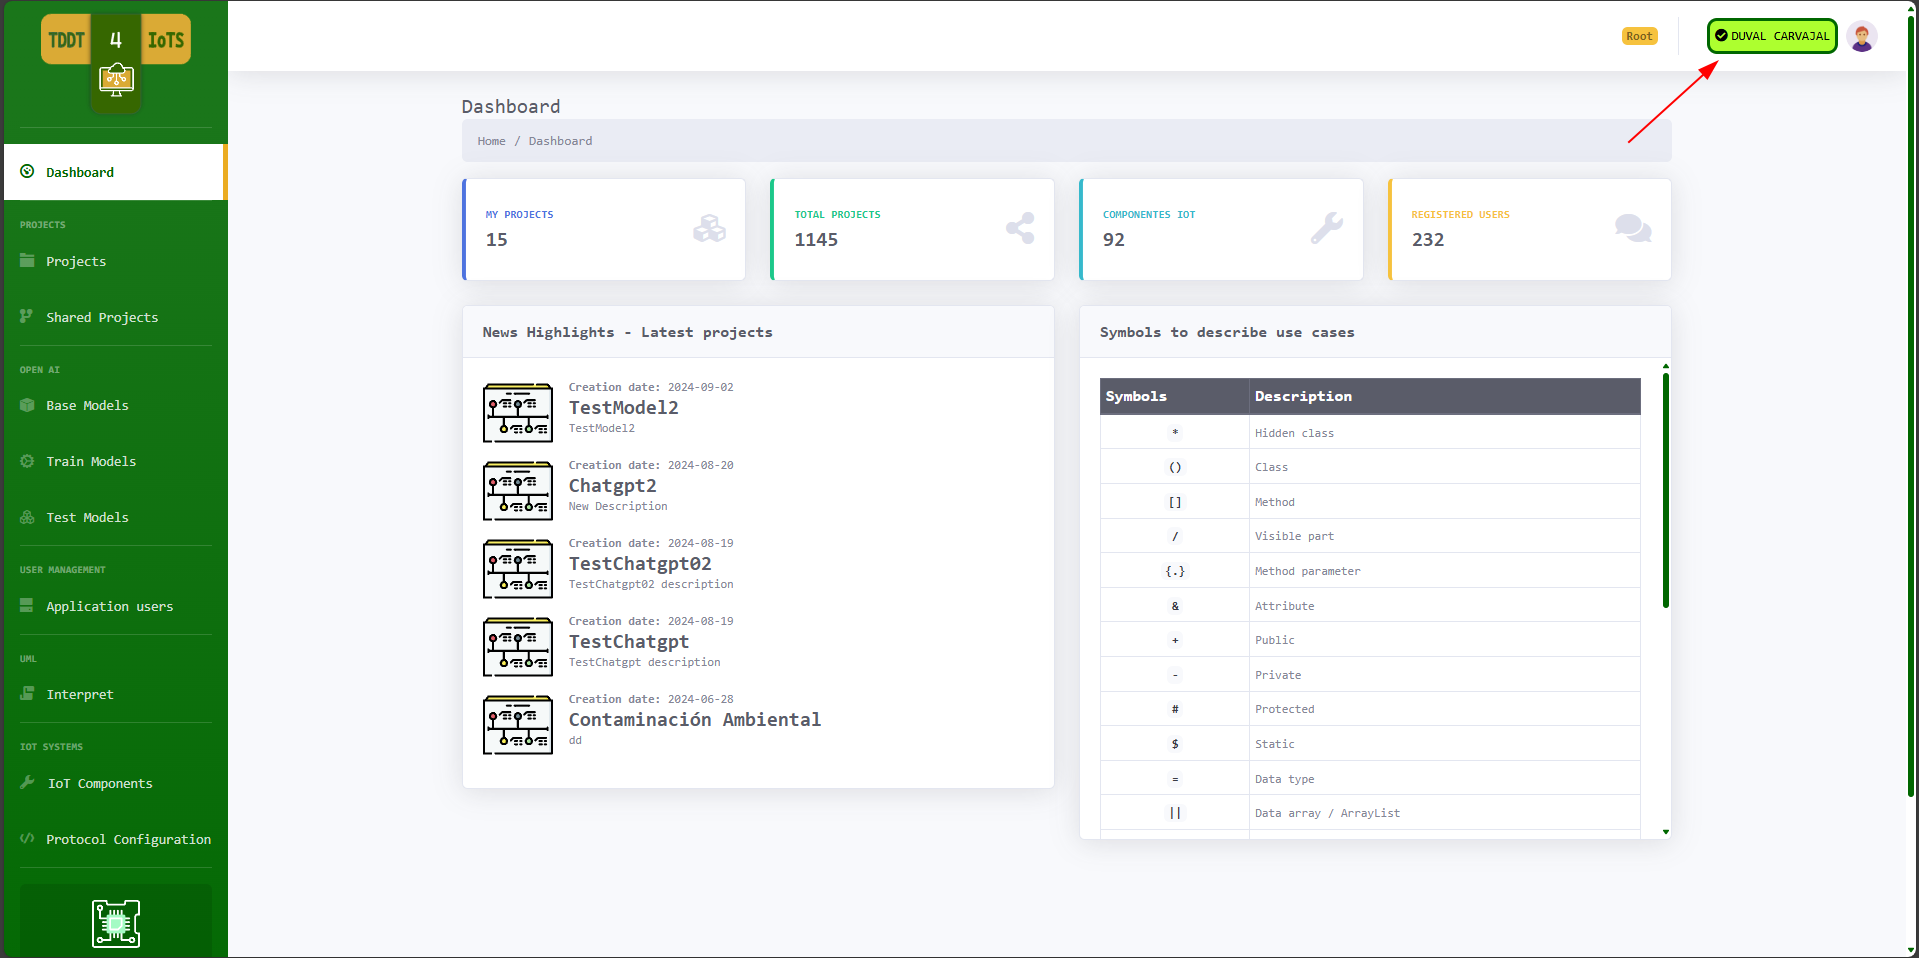
\includegraphics[width=\textwidth]{interfaz001.png}
	\caption{Interfaz principal de la aplicación.}
	\label{fig:cap3_interfaz_001}
\end{figure}

La figura \ref{fig:cap3_interfaz_002} muestra las nuevas opciones que se despliegan al dar click en el nombre de usuario. La opción \textit{"Secret Key OpenAI"} permite poder ingresar la clave secreta de la API de OpenAI.

\begin{figure}[H]  
	\centering
	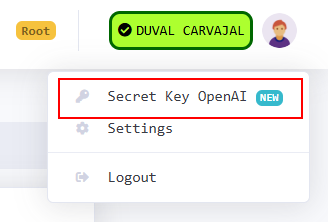
\includegraphics[width=170px]{interfaz002.png} 
	\caption{Opción para agregar la clave secreta de la API de OpenAI.}
	\label{fig:cap3_interfaz_002}
\end{figure}

En la figura \ref{fig:cap3_interfaz_003} se observa el formulario que aparecerá cuando ingresemos a la opción de \textit{"Secret Key OpenAI"}.

\begin{figure}[H]  
	\centering
	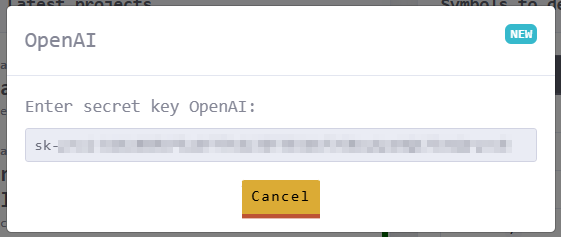
\includegraphics[width=240px]{interfaz003.png} 
	\caption{Formulario para ingresar la clave secreta de OpenAi.}
	\label{fig:cap3_interfaz_003}
\end{figure}

La figura \ref{fig:cap3_interfaz_004} muestra en en el recuadro rojo la opción para configurar los modelos de OpenAI disponibles dentro de la herramienta.
 
\begin{figure}[H]  
	\centering
	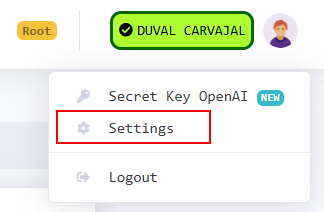
\includegraphics[width=140px]{interfaz004.png} 
	\caption{Opcion para configurar la API de OpenAI.}
	\label{fig:cap3_interfaz_004}
\end{figure}

Al acceder a la opción de \textit{``Settings"}, aparece un formulario que está dividido en dos secciones (ver figura \ref{fig:cap3_interfaz_005}). La opción de \textit{``OpenAI"} muestra los modelos disponibles en la herramienta. 

\begin{figure}[H]  
\centering
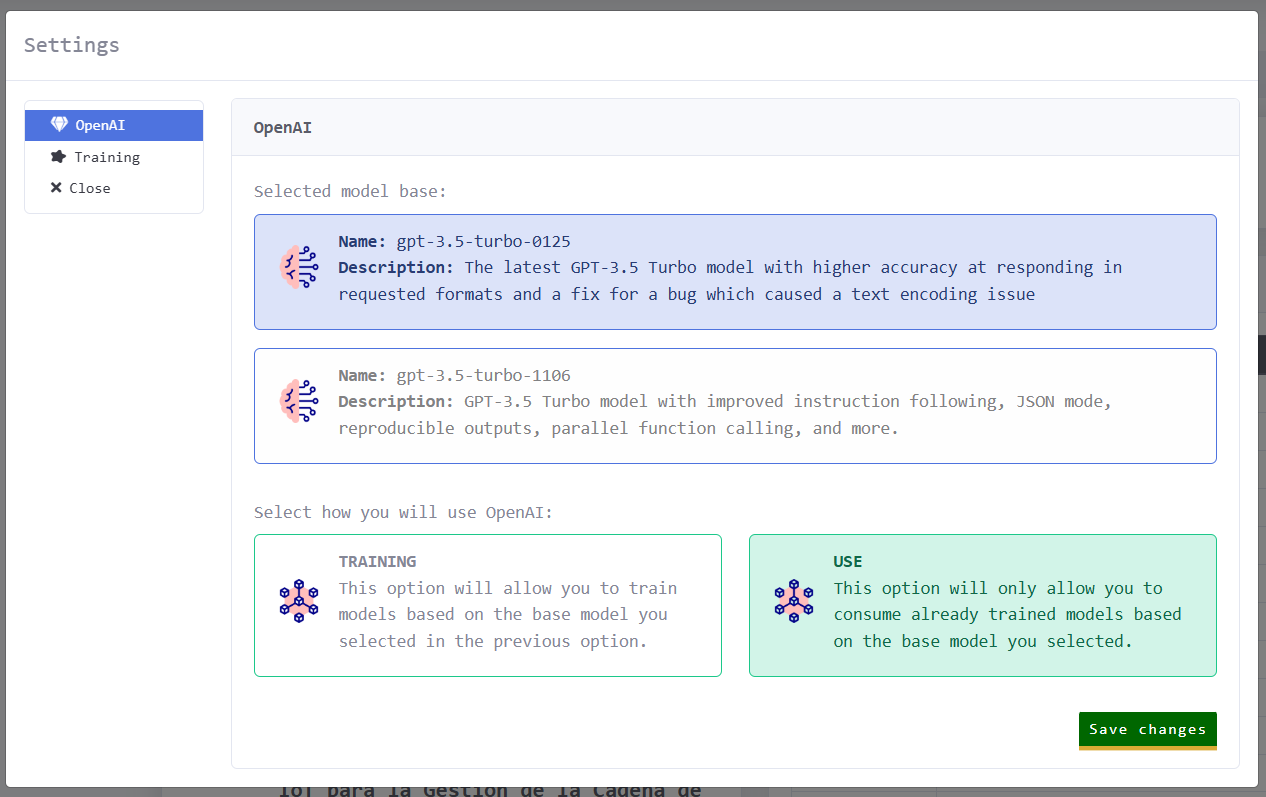
\includegraphics[width=300px]{interfaz005.png} 
\caption{Formulario de configuración de los modelos de OpenAi. Modelos base y el uso que le dará el usuario.}
\label{fig:cap3_interfaz_005}
\end{figure}

En la primera subsección, se visualizan los modelos base de la herramienta, destacándose en color azul el modelo base que ha sido seleccionado por el usuario. En la segunda subsección, se muestra el tipo de uso que el usuario está aplicando al modelo. En este caso, el modelo base seleccionado está siendo utilizado específicamente para interpretar el texto natural enviado a través de las descripciones de los casos de uso.

La sección de \textit{``Training"} muestra la información sobre los entrenamientos realizados sobre le modelo base que se encuentra seleccionado. Además, se observa el nombre del usuario quien realizo el entrenamiento respectivo al modelo (ver figura \ref{fig:cap3_interfaz_006}).

\begin{figure}[H]  
 	\centering
 	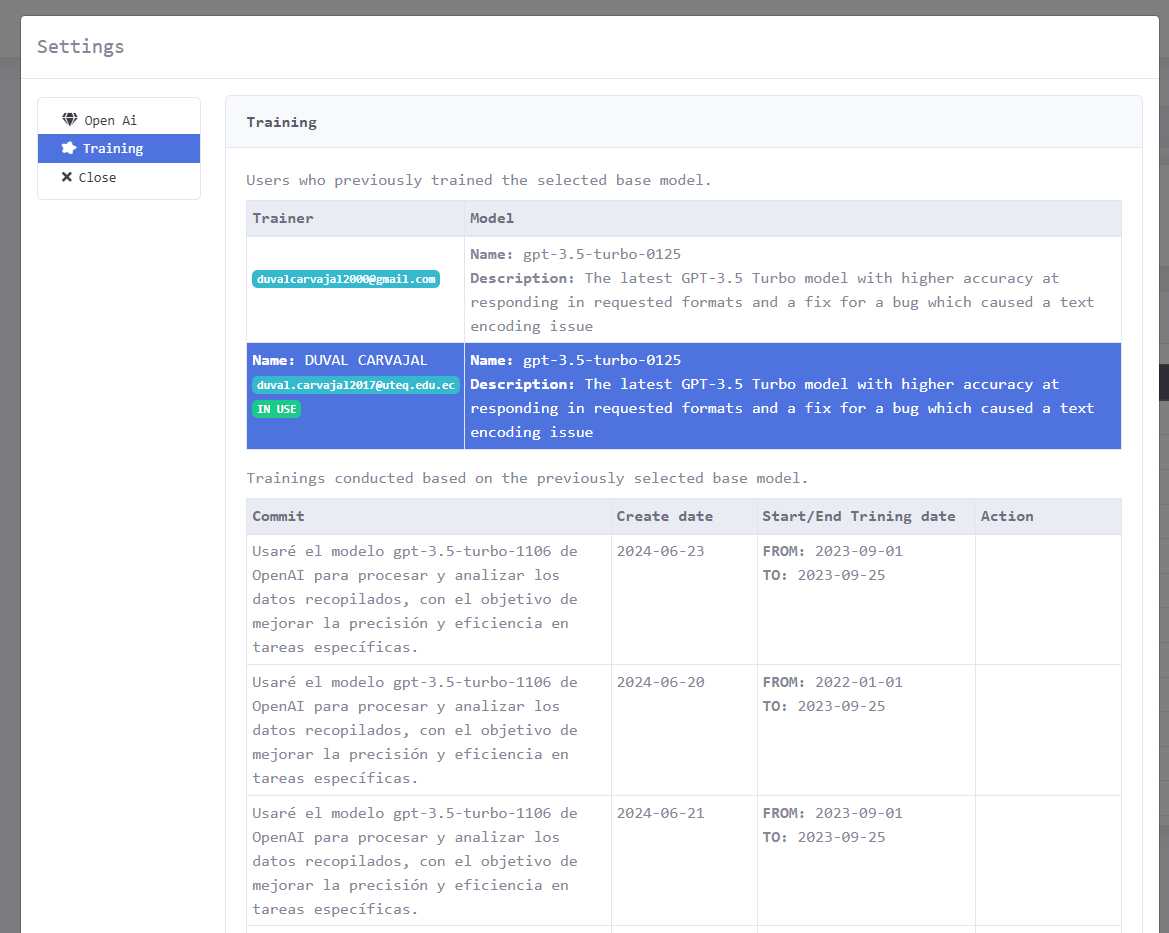
\includegraphics[width=\textwidth]{interfaz006.png} 
 	\caption{Formulario de configuración de los modelos de OpenAi. Entrenamiento de los modelos base y su modelo seleccionado.}
 	\label{fig:cap3_interfaz_006}
\end{figure}

Dentro de la herramienta se agregaron 3 opciones al menú principal con el objetivo de gestionar los modelos base que podrán ser ingresados, los entrenamientos y una ultima opción para poder probar el modelo entrenado de forma independiente a los proyectos que tenga la herramienta. La figura \ref{fig:cap3_interfaz_008} muestra la opción \textit{``Base Models"} que permitirá ingresar los modelos base de OpenAi que se crean necesarios para ser utilizados por la herramienta.

\begin{figure}[H]  
	\centering
	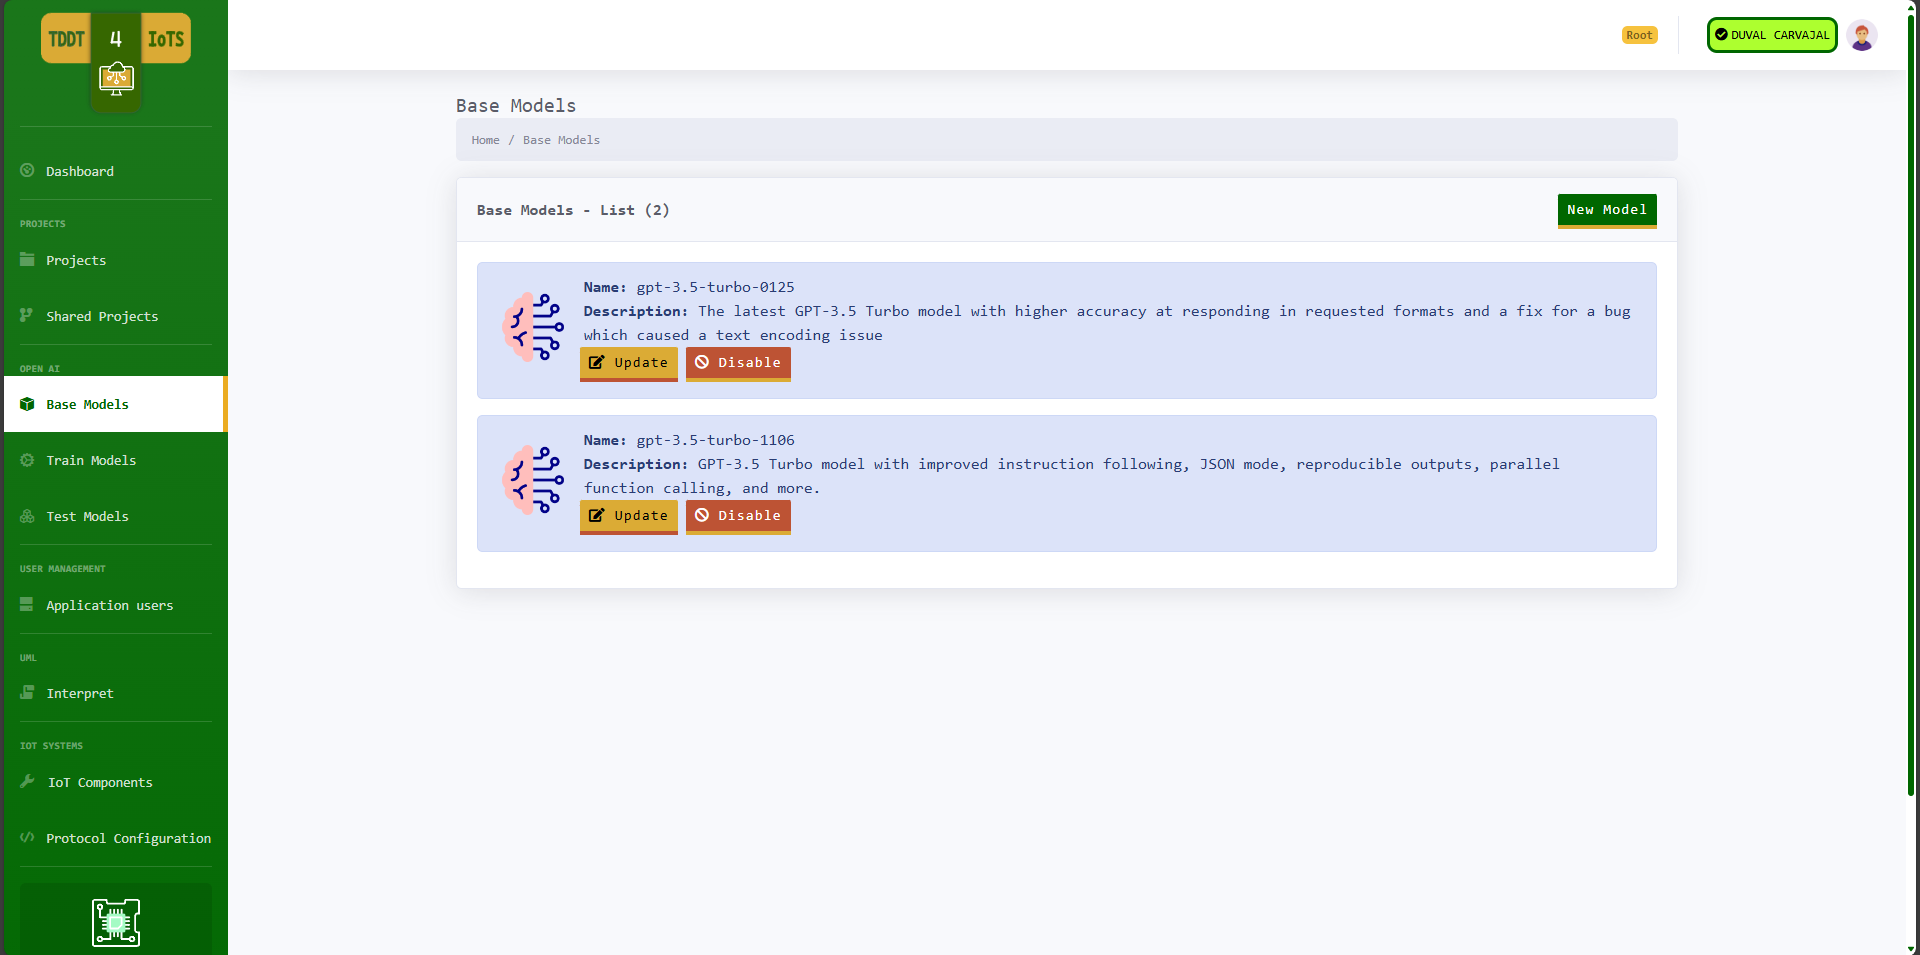
\includegraphics[width=300px]{interfaz008.png} 
	\caption{Opción para gestionar los modelos base de OpenAI dentro de la herramienta.}
	\label{fig:cap3_interfaz_008}
\end{figure}

La figura \ref{fig:cap3_interfaz_009} muestra la opción \textit{``Train models"}. En esta opción se podrán gestionar los entrenamientos al modelo base seleccionado. Se puede observar una lista de los entrenamientos y el estado en el que se encuentra o quedo cada entrenamiento que fue realizado desde la herramienta. Los datos para el entrenamiento son en base a los datos que actualmente se encontraron en la herramienta.  

\begin{figure}[H]  
	\centering
	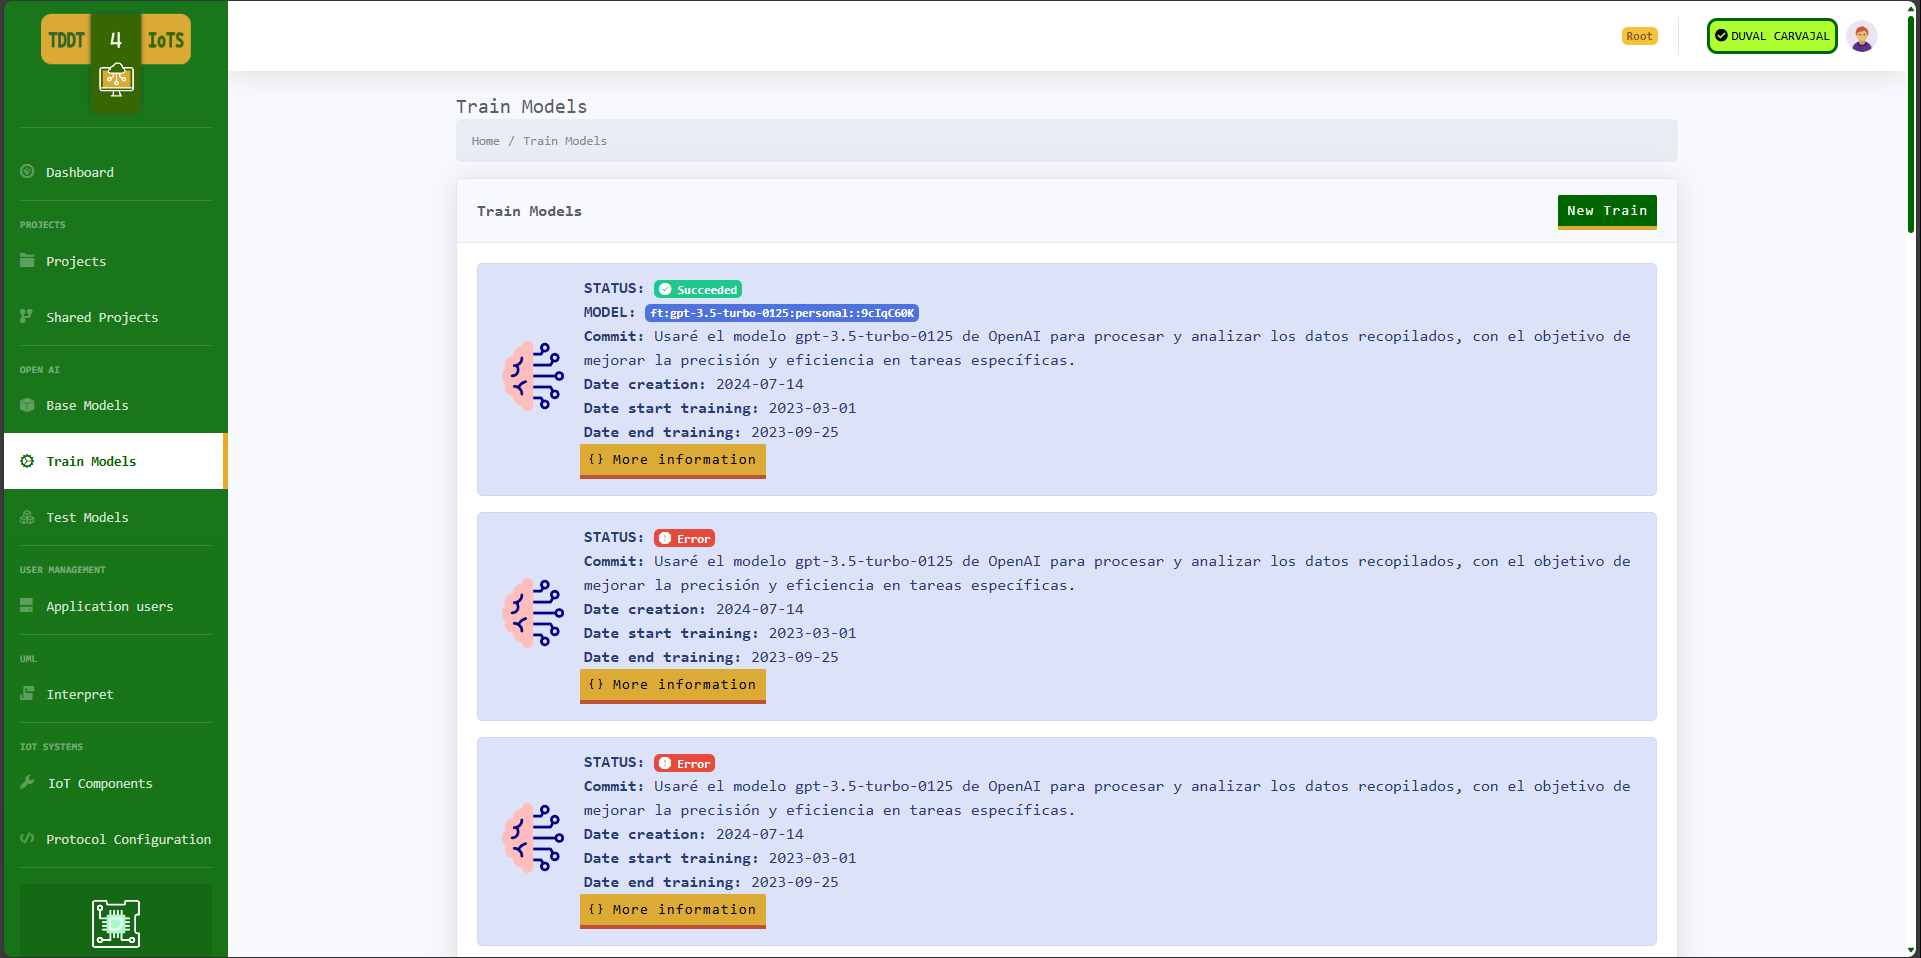
\includegraphics[width=300px]{interfaz009.png} 
	\caption{Opción para gestionar los entrenamientos de los modelos base de OpenAI dentro de la herramienta.}
	\label{fig:cap3_interfaz_009}
\end{figure} 

Para conocer mas información detallada sobre cada entrenamiento realizado, se puede ingresar a la opción de \textit{"More information"} (ver figura \ref{fig:cap3_interfaz_010}). Al ingresar a esa opción en la figura \ref{fig:cap3_interfaz_011} se observa  como se desplegara un formulario con el \textit{JSON} de respuesta devuelto por OpenAI del entrenamiento realizado. 

\begin{figure}[H]  
	\centering
	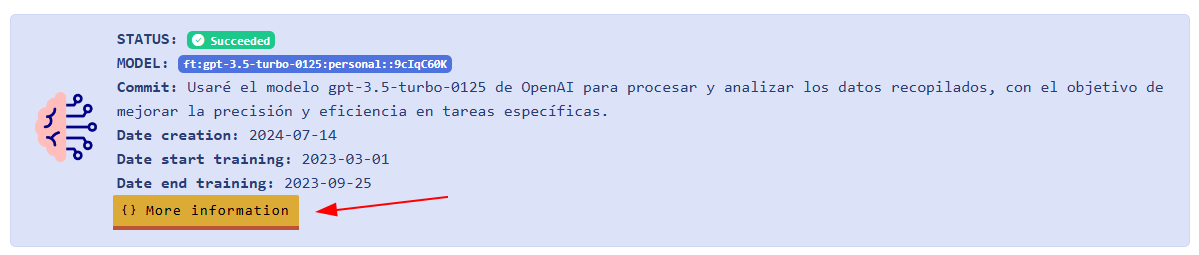
\includegraphics[width=300px]{interfaz010.png} 
	\caption{Estado de un entrenamiento realizado dentro de la herramienta y sus opciones disponibles.}
	\label{fig:cap3_interfaz_010}
\end{figure} 

\begin{figure}[H]  
	\centering
	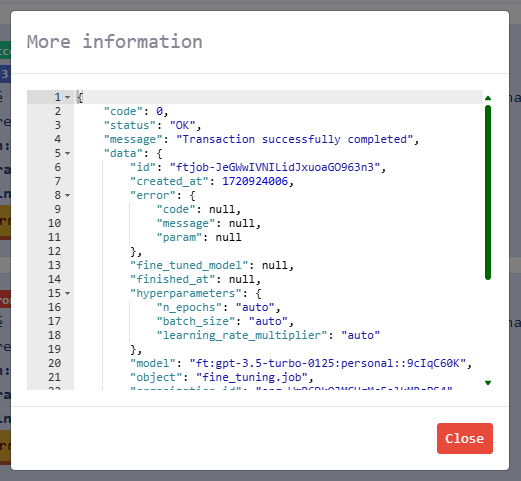
\includegraphics[width=250px]{interfaz011.png} 
	\caption{Información detallada del entrenamiento.}
	\label{fig:cap3_interfaz_011}
\end{figure}

La figura \ref{fig:cap3_interfaz_012} muestra la última opción denominada \textit{``Test Models"}. Esta opción permite al usuario probar el modelo seleccionado para utilizarlo dentro de la herramienta \textit{case}. Para realizar la prueba, solo se requiere proporcionar un texto en lenguaje natural que describa una parte de los casos de uso del sistema informático qeu se esté desarrollando en ese momento mediante la herramienta. Luego, se espera la respuesta de OpenAI, y la herramienta genera el diagrama de clases correspondiente según la solicitud descrita en el texto enviado.
 
 \begin{figure}[H]  
 	\centering
 	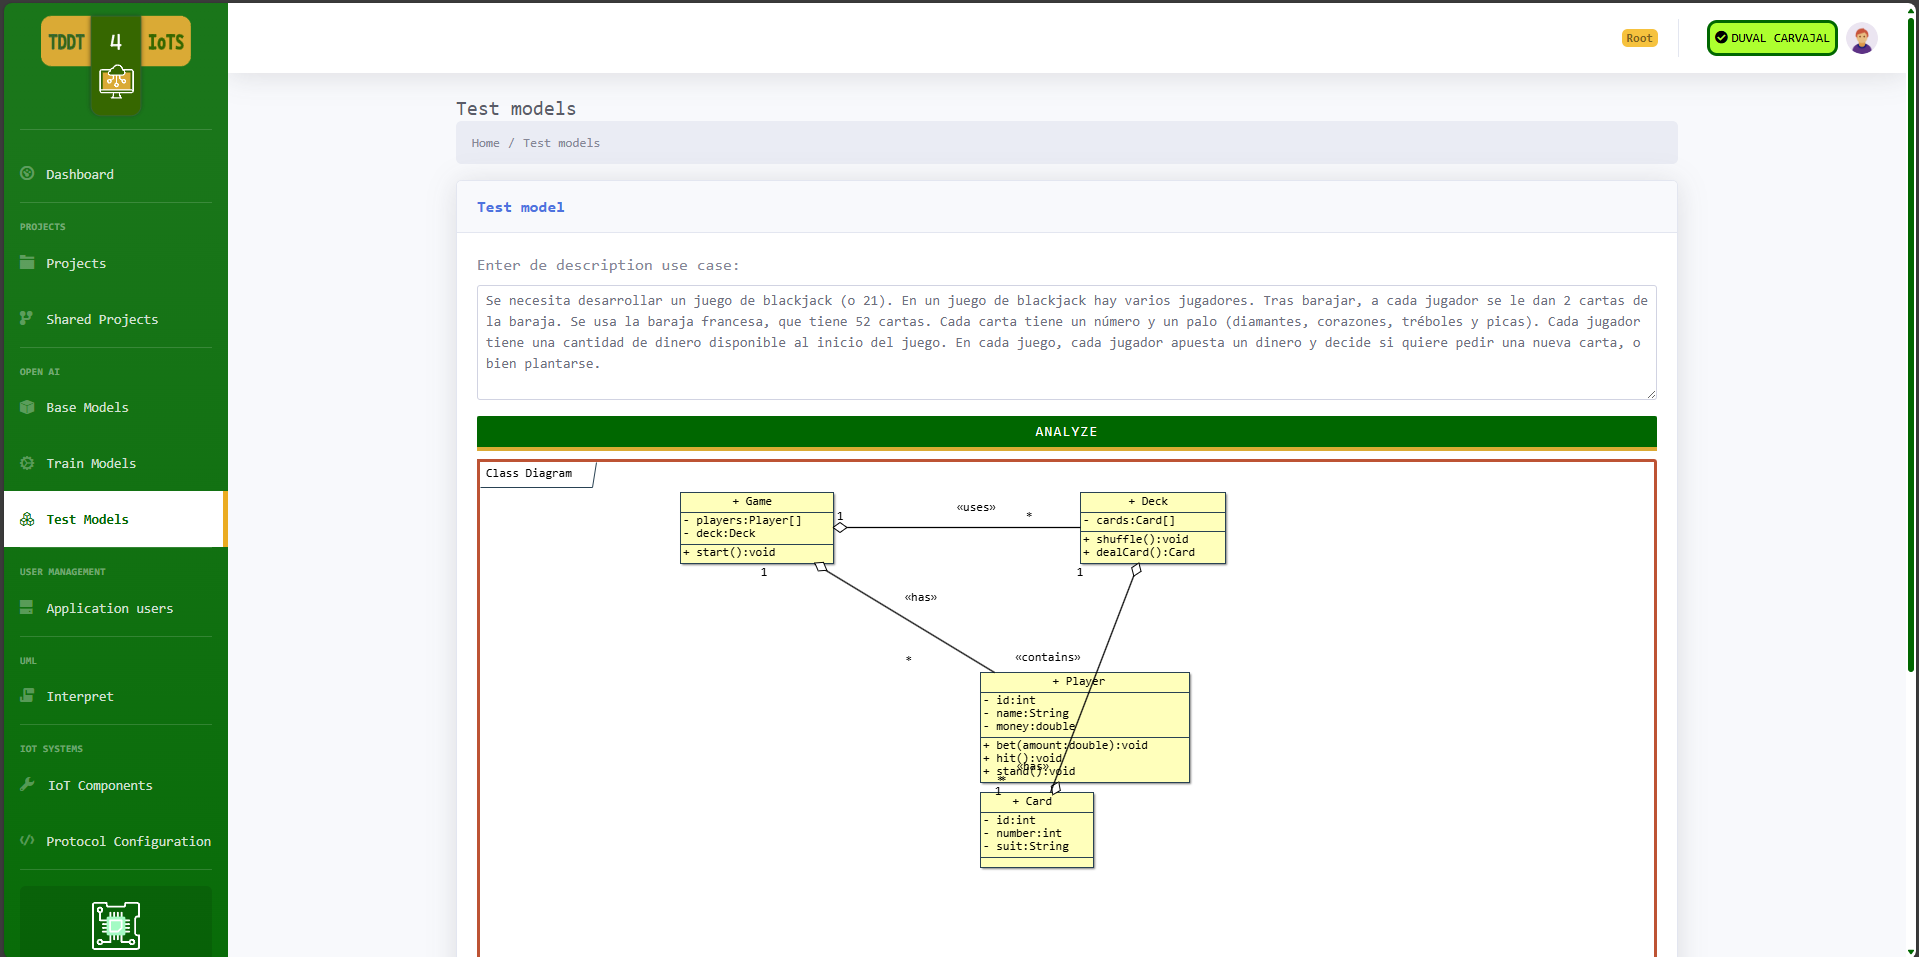
\includegraphics[width=\textwidth]{interfaz012.png} 
 	\caption{Prueba del modelo de OpenAI entrenado.}
 	\label{fig:cap3_interfaz_012}
 \end{figure}

Una vez que el modelo entrenado esté listo y se haya comprobado que puede analizar correctamente la descripción del caso de uso enviado, se puede proceder a la siguiente etapa de la herramienta. En esta etapa, se utilizará el modelo con todas las descripciones de los casos de uso del sistema de interés para generar un diagrama de clases lo más ajustado al objetivo del sistema a desarrollar. En la figura \ref{fig:cap3_interfaz_013}, se muestra cómo la flecha señala una opción denominada \textit{``Activate OpenAI"}. Permite activar o desactivar el uso del modelo para analizar las descripciones de los casos de uso. Dado que la herramienta incluye un intérprete de descripciones de casos de uso, esta opción determina si se desea emplear el modelo en el análisis o no.


 \begin{figure}[H]  
	\centering
	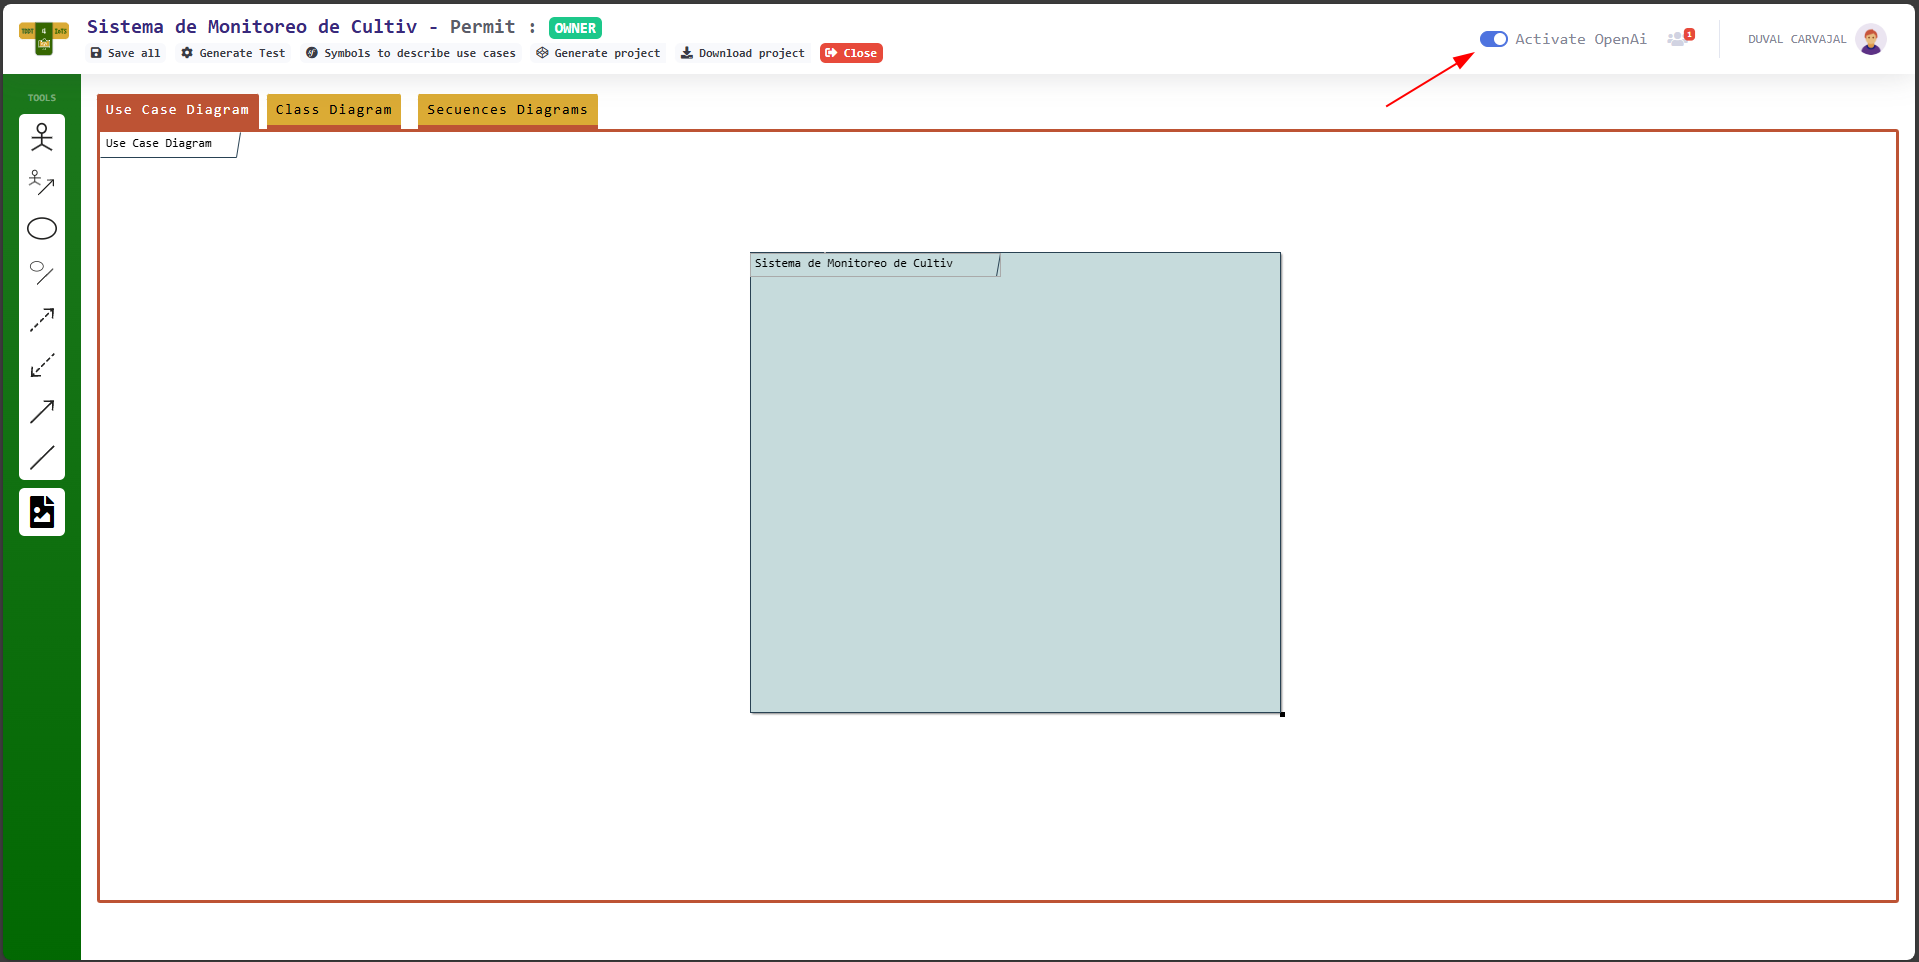
\includegraphics[width=\textwidth]{interfaz013.png} 
	\caption{Área para crear un diagrama de casos de uso e indicar si se usara el modelo de OpenAI.}
	\label{fig:cap3_interfaz_013}
\end{figure}

La figura \ref{fig:cap3_interfaz_014} muestra como la descripción del caso de uso actual esta ingresada con texto natural. Esperando que el modelo sea capaz de interpretar cada sección del caso de uso y también todos los casos de uso que permitan crear el diagrama de clases. 

 \begin{figure}[H]  
	\centering
	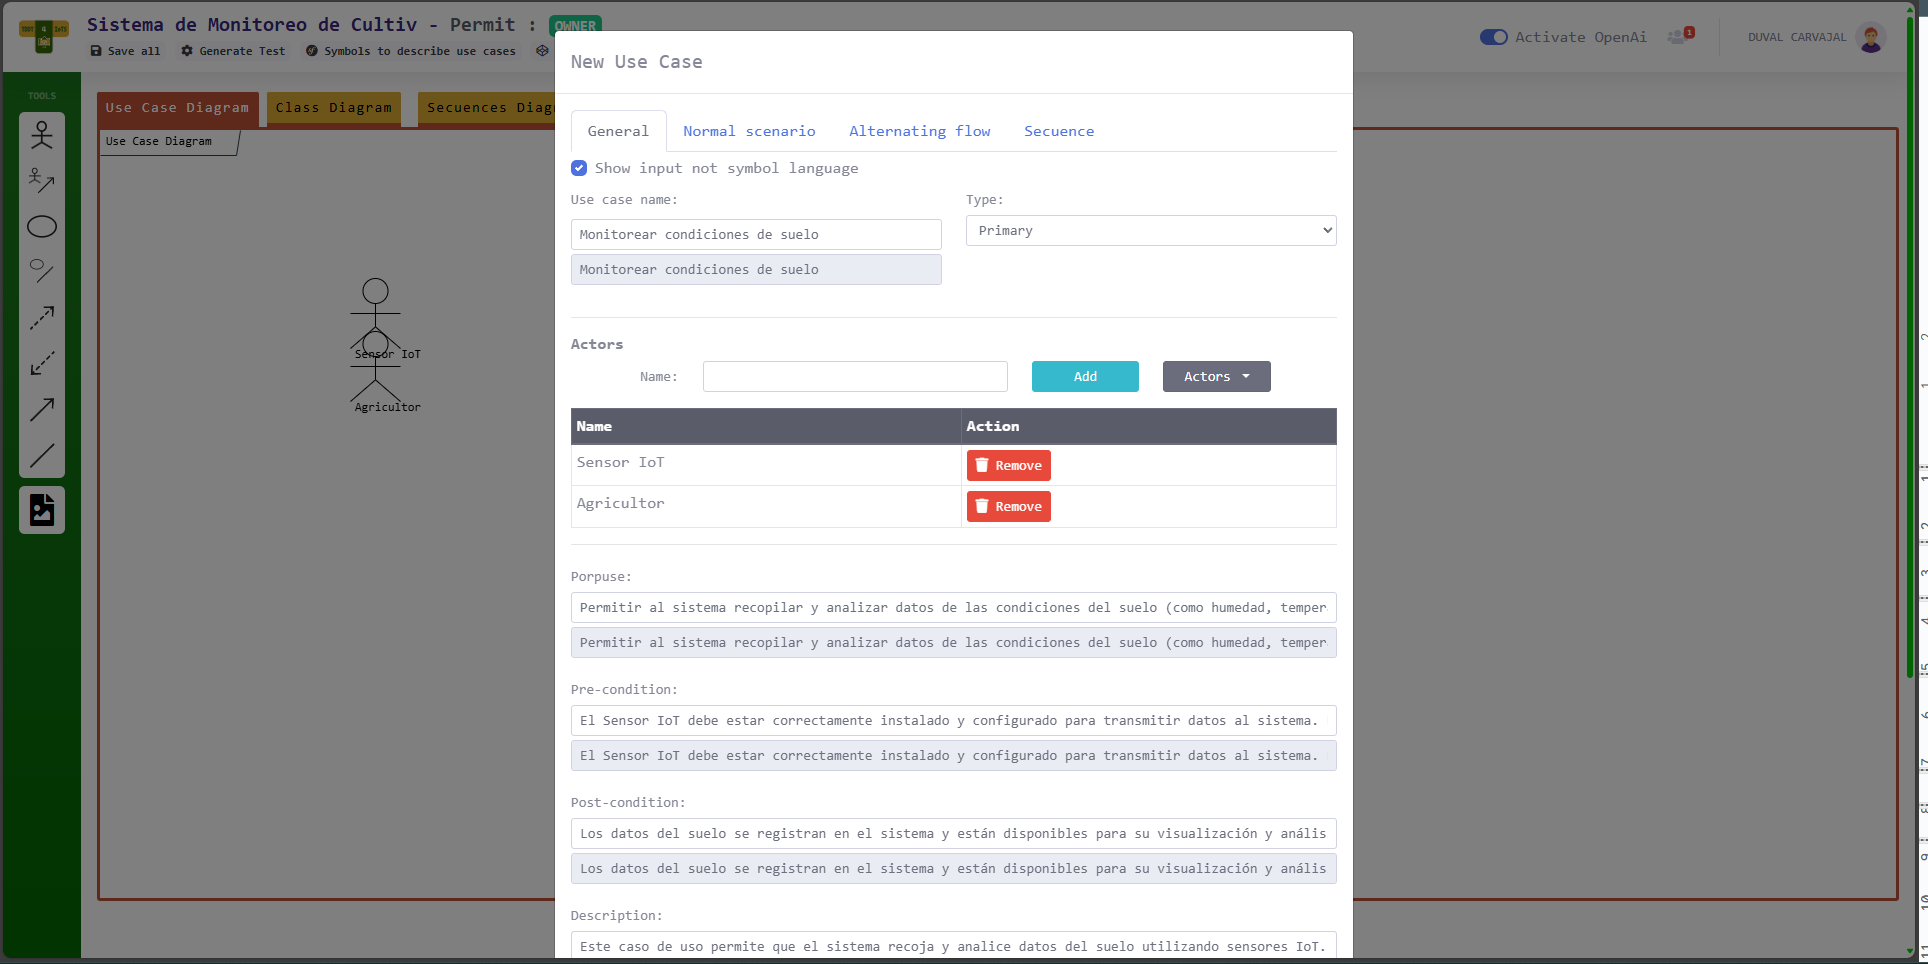
\includegraphics[width=\textwidth]{interfaz014.png} 
	\caption{Formulario para ingresar la descripción de cada caso de uso del sistema.}
	\label{fig:cap3_interfaz_014}
\end{figure}

Cuando el modelo este trabajando sobre los casos de uso se podrá observar una leyenda que indicara el momento que OpenAI está analizando las descripciones de los casos de uso (ver figura \ref{fig:cap3_interfaz_015}). 

 \begin{figure}[H]  
	\centering
	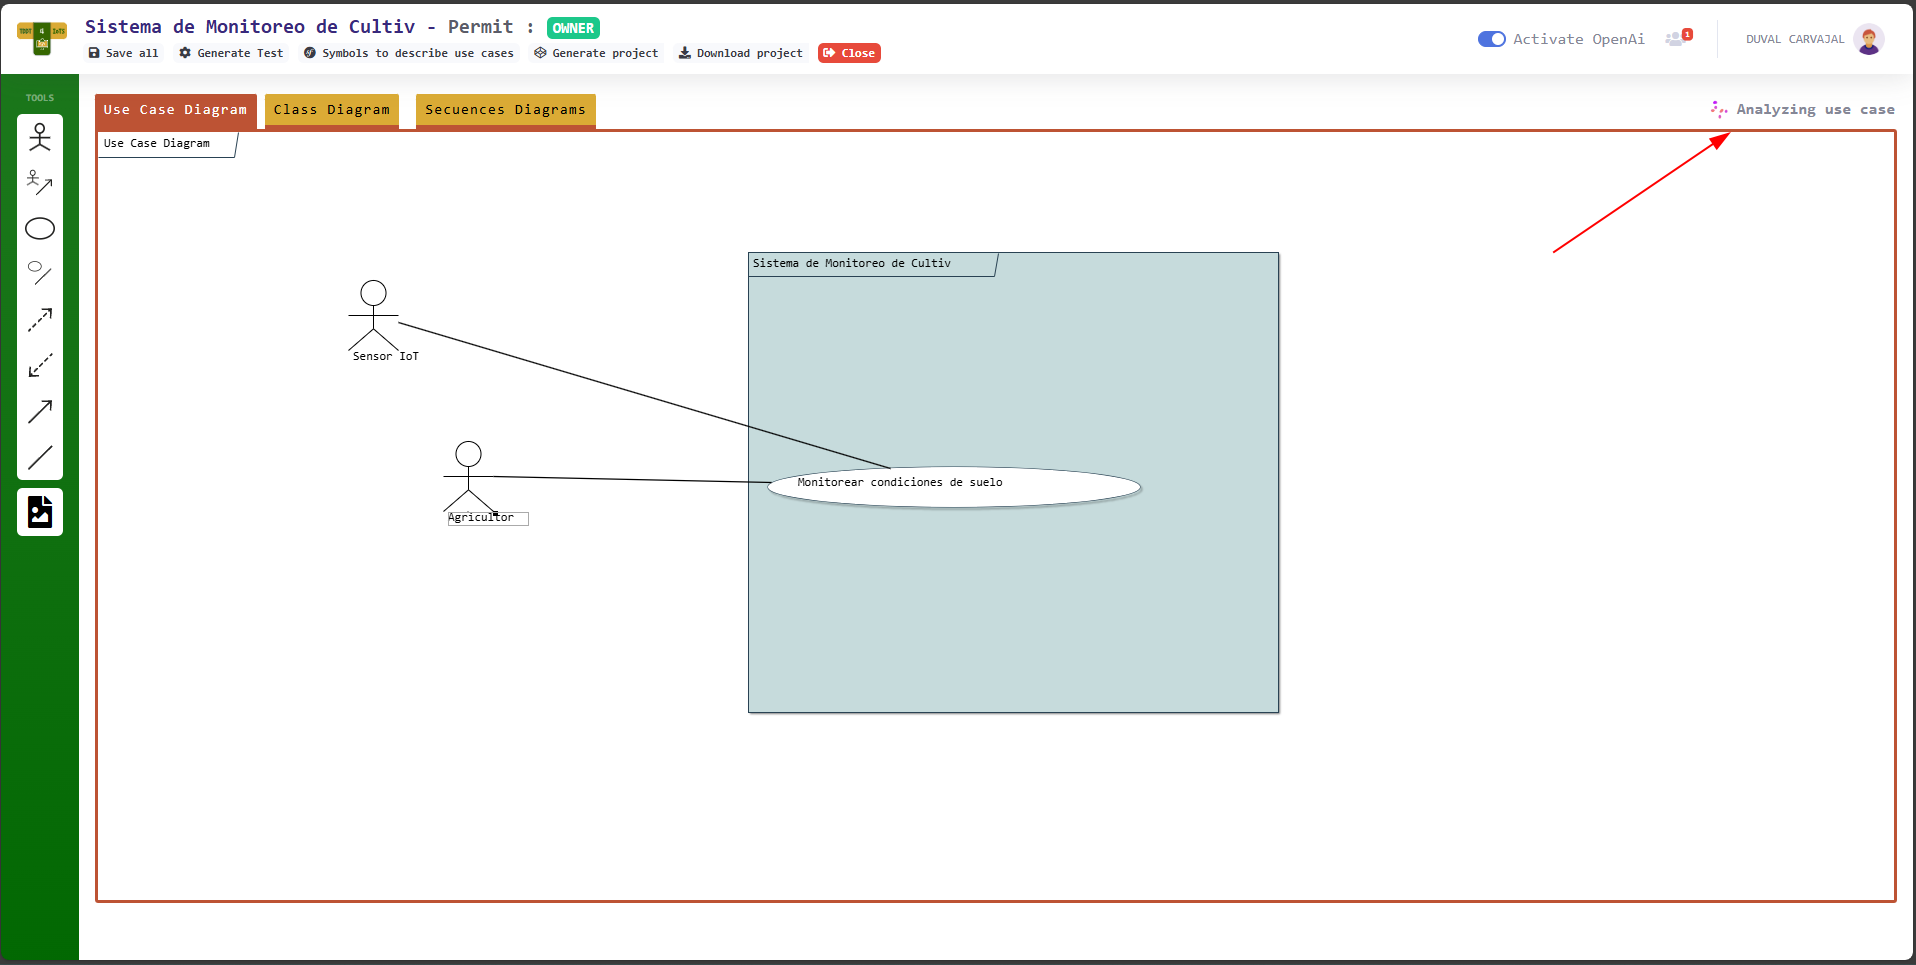
\includegraphics[width=\textwidth]{interfaz015.png} 
	\caption{Estado del modelo al analizar los casos de uso.}
	\label{fig:cap3_interfaz_015}
\end{figure}

Finalmente, en la figura \ref{fig:cap3_interfaz_016} se muestra como la herramienta fue capaz de generar el diagrama de clases mediante las descripciones de los casos de uso del sistema a desarrollar.

 \begin{figure}[H]  
	\centering
	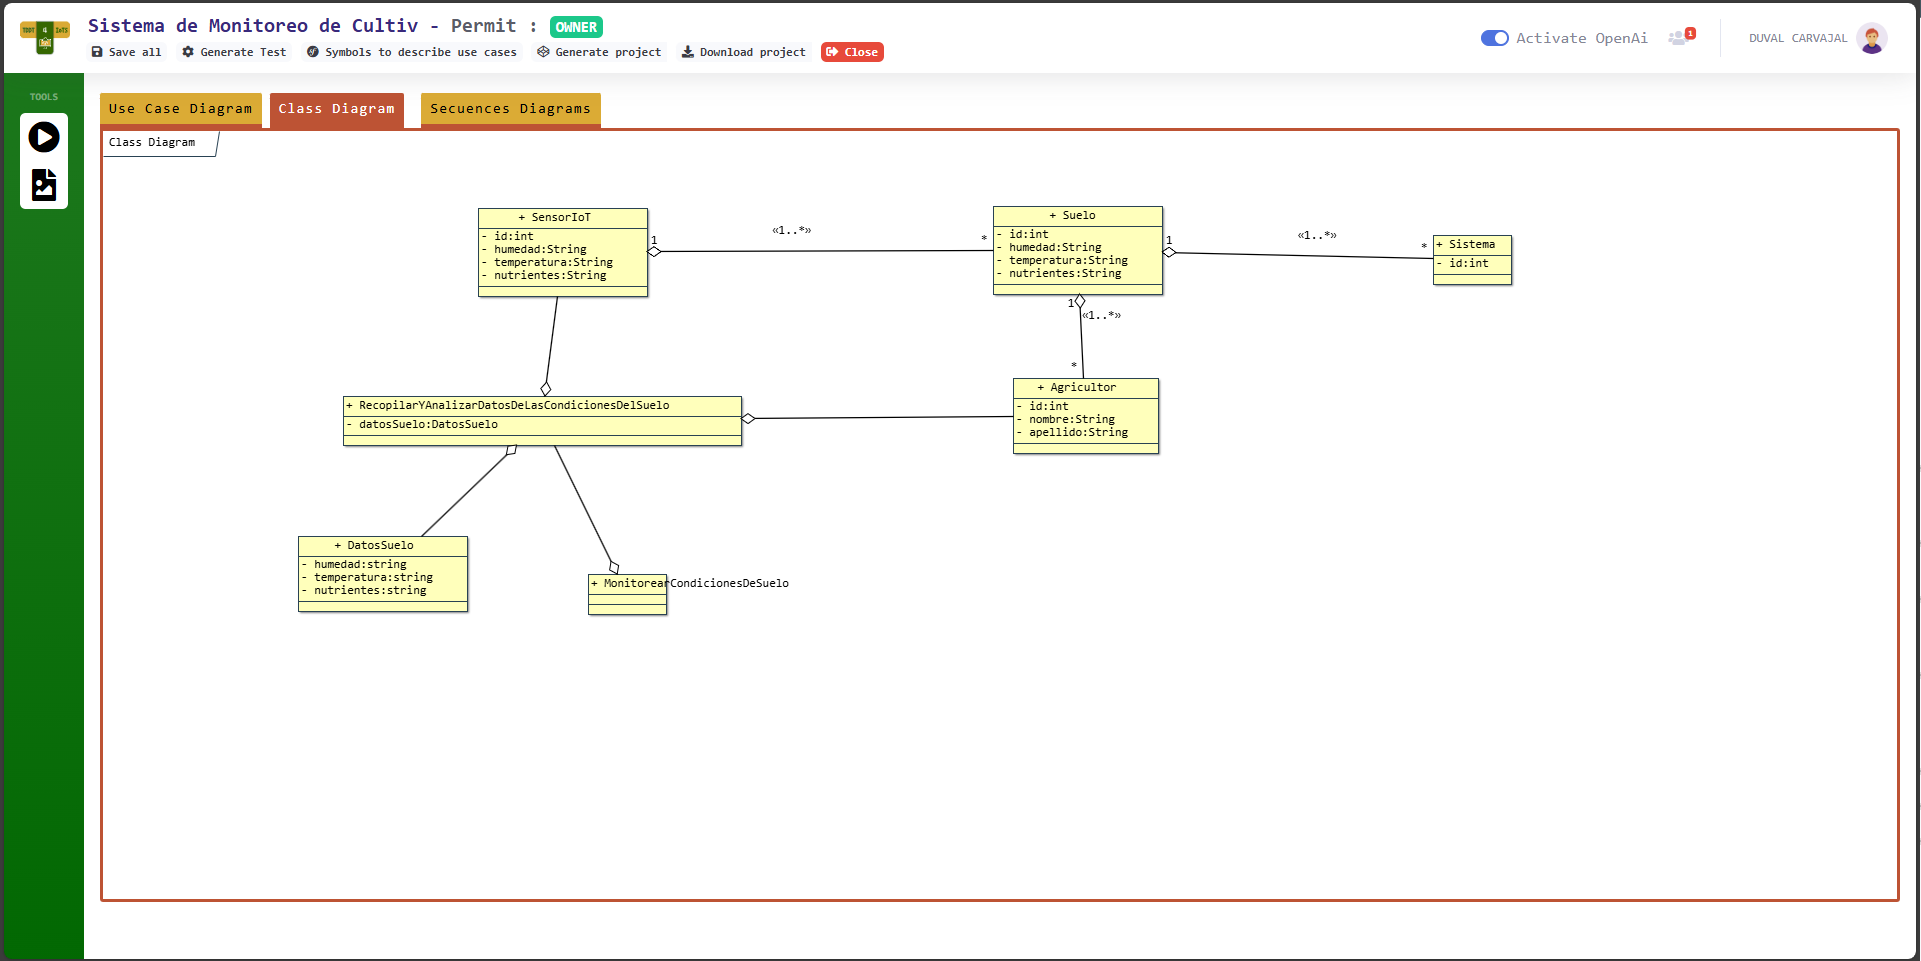
\includegraphics[width=\textwidth]{interfaz016.png} 
	\caption{Diagrama de clases generado por la herramienta y el modelo de OpenAI.}
	\label{fig:cap3_interfaz_016}
\end{figure}

\subsection{Evaluación de la extensión dentro de la aplicación web}

Para evaluar la efectividad de la herramienta, se contactó con 15 estudiantes de la Universidad Técnica Estatal de Quevedo, Ecuador. A estos estudiantes se les solicitó que utilizaran la herramienta y cargaran uno de los proyectos en los que estuvieran trabajando durante sus estudios, creando el diagrama de casos de uso para su sistema IoT. Una vez redactadas las descripciones de los casos de uso en lenguaje natural, la herramienta analizó cada proyecto y genero automáticamente el diagrama de clases correspondiente para cada proyecto.

A cada estudiante se le envió la invitación a un documento compartido para que pudieran ingresar las descripciones de los casos de uso y tener documentado todos los proyectos que se ingresaron en la herramienta para su respectiva evaluación. En el siguiente enlace (\url{https://acortar.link/pqSAZi}) se muestra el documento de texto que fue compartido y se observan las descripciones de los casos de uso de cada proyecto.

Para las descripciones de los casos de uso se les indico una plantilla para que puedan documentarla y sea mas fácil ingresarlos dentro de la herramienta. 

\subsection{Ejemplo de proyecto usado para evaluar la extensión de la herramienta}

A continuación se mostrará un ejemplo de uno de los proyectos evaluados.

\textbf{Proyecto: } Sistema de Monitoreo de Cultivos Inteligente con IoT \\
\textbf{Descripción: } Desarrollo de una red de sensores IoT para monitorear condiciones del suelo, humedad y temperatura en cultivos, optimizando el riego y mejorando la productividad agrícola. 

\begin{longtable}{|p{5cm}|p{5cm}|}
	\hline
	\multicolumn{2}{|c|}{\textbf{Caso de uso: Monitorizar condiciones de suelo}} \\
	\hline
	\textbf{Tipo:} & Primario \\
	\hline
	\textbf{Actores:} & Sensor IoT, Agricultor \\
	\hline
	\textbf{Propósito:} & Permitir al sistema recopilar y analizar datos de las condiciones del suelo (como humedad, temperatura y nutrientes) para ayudar en la toma de decisiones del agricultor. \\
	\hline
	\textbf{Precondición:} & El Sensor IoT debe estar correctamente instalado y configurado para transmitir datos al sistema. El agricultor debe tener acceso al sistema. \\
	\hline
	\textbf{Postcondición:} & Los datos del suelo se registran en el sistema y están disponibles para su visualización y análisis. \\
	\hline
	\textbf{Descripción:} & Este caso de uso permite que el sistema recoja y analice datos del suelo utilizando sensores IoT. Los datos recopilados son accesibles para el agricultor en tiempo real, y se pueden usar para la toma de decisiones sobre el manejo de los cultivos. \\
	\hline
	\multicolumn{2}{|c|}{\textbf{Flujo normal}} \\
	\hline
	\textbf{Actor} & \textbf{Sistema} \\
	\hline
	1. El Sensor IoT recopila datos del suelo en intervalos regulares. & \\
	\hline
	& 2. El sistema recibe y almacena los datos. \\
	\hline
	& 3. El sistema analiza los datos para detectar patrones o tendencias. \\
	\hline
	4. El agricultor puede acceder a los datos en tiempo real a través del sistema. & \\
	\hline
	\multicolumn{2}{|c|}{\textbf{Flujo alternativo}} \\
	\hline
	\textbf{Actor} & \textbf{Sistema} \\
	\hline
	1. Si el Sensor IoT no puede transmitir los datos, el sistema genera una notificación al agricultor para tomar acciones correctivas. & \\
	\hline
\end{longtable}

\begin{longtable}{|p{5cm}|p{5cm}|}
	\hline
	\multicolumn{2}{|c|}{\textbf{Caso de uso: Notificar anomalías}} \\
	\hline
	\textbf{Tipo:} & Primario \\
	\hline
	\textbf{Actores:} & Agricultor \\
	\hline
	\textbf{Propósito:} & Informar al agricultor sobre cualquier condición anómala detectada en el suelo para que pueda tomar medidas inmediatas. \\
	\hline
	\textbf{Precondición:} & El sistema debe estar monitoreando las condiciones del suelo activamente y contar con una base de datos de condiciones normales. \\
	\hline
	\textbf{Postcondición:} & El agricultor es informado de la anomalía y puede tomar acciones correctivas. \\
	\hline
	\textbf{Descripción:} & El sistema detecta automáticamente cualquier condición anómala en el suelo y notifica al agricultor para que pueda actuar rápidamente. Este proceso asegura que el agricultor esté siempre informado de posibles problemas que puedan afectar sus cultivos. \\
	\hline
	\multicolumn{2}{|c|}{\textbf{Flujo normal}} \\
	\hline
	\textbf{Actor} & \textbf{Sistema} \\
	\hline
	& 1. El sistema detecta una condición anómala en los datos del suelo (ej. baja humedad, presencia de plagas). \\
	\hline
	& 2. El sistema genera una notificación automática. \\
	\hline
	3. El agricultor recibe la notificación en su dispositivo. & \\
	\hline
	\multicolumn{2}{|c|}{\textbf{Flujo alternativo}} \\
	\hline
	\textbf{Actor} & \textbf{Sistema} \\
	\hline
	1. Si el agricultor no responde a la notificación, el sistema envía recordatorios o escala la notificación a otros medios (como SMS). & \\
	\hline
\end{longtable}

\begin{longtable}{|p{5cm}|p{5cm}|}
	\hline
	\multicolumn{2}{|c|}{\textbf{Caso de uso: Visualizar datos en tiempo real}} \\
	\hline
	\textbf{Tipo:} & Primario \\
	\hline
	\textbf{Actores:} & Agricultor \\
	\hline
	\textbf{Propósito:} & Permitir al agricultor acceder a una interfaz que muestre los datos actuales de las condiciones del suelo, facilitando el monitoreo continuo. \\
	\hline
	\textbf{Precondición:} & El sistema debe estar recibiendo y procesando datos del Sensor IoT en tiempo real. \\
	\hline
	\textbf{Postcondición:} & Los datos se muestran correctamente y están actualizados en la interfaz del usuario. \\
	\hline
	\textbf{Descripción:} & El agricultor puede monitorear las condiciones del suelo en tiempo real mediante una interfaz visual proporcionada por el sistema, lo que le permite tomar decisiones informadas sobre el manejo de sus cultivos. \\
	\hline
	\multicolumn{2}{|c|}{\textbf{Flujo normal}} \\
	\hline
	\textbf{Actor} & \textbf{Sistema} \\
	\hline
	1. El agricultor accede al sistema a través de su dispositivo. & \\
	\hline
	& 2. El sistema muestra los datos en una interfaz gráfica en tiempo real. \\
	\hline
	3. El agricultor puede observar y analizar los datos para tomar decisiones inmediatas. & \\
	\hline
	\multicolumn{2}{|c|}{\textbf{Flujo alternativo}} \\
	\hline
	\textbf{Actor} & \textbf{Sistema} \\
	\hline
	1. Si la conexión con el Sensor IoT falla, el sistema muestra una advertencia y proporciona los últimos datos disponibles. & \\
	\hline
\end{longtable}

\begin{longtable}{|p{5cm}|p{5cm}|}
	\hline
	\multicolumn{2}{|c|}{\textbf{Caso de uso: Automatizar riego}} \\
	\hline
	\textbf{Tipo:} & Primario \\
	\hline
	\textbf{Actores:} & Agricultor \\
	\hline
	\textbf{Propósito:} & Automatizar el proceso de riego basado en los datos del suelo, optimizando el uso de agua y asegurando que las plantas reciban la cantidad adecuada de humedad. \\
	\hline
	\textbf{Precondición:} & El sistema debe tener acceso a un controlador de riego automatizado y los datos del Sensor IoT deben estar disponibles. \\
	\hline
	\textbf{Postcondición:} & El riego se activa o desactiva automáticamente según las condiciones del suelo. \\
	\hline
	\textbf{Descripción:} & Este caso de uso permite al sistema tomar decisiones automatizadas sobre el riego de cultivos basándose en los datos del suelo, optimizando así los recursos hídricos y garantizando la salud de las plantas. \\
	\hline
	\multicolumn{2}{|c|}{\textbf{Flujo normal}} \\
	\hline
	\textbf{Actor} & \textbf{Sistema} \\
	\hline
	& 1. El sistema analiza los datos del Sensor IoT y determina si el suelo necesita riego. \\
	\hline
	& 2. Si se requiere riego, el sistema activa el sistema de riego automatizado. \\
	\hline
	& 3. El sistema monitorea el riego y lo detiene una vez que se alcanzan las condiciones óptimas. \\
	\hline
	\multicolumn{2}{|c|}{\textbf{Flujo alternativo}} \\
	\hline
	\textbf{Actor} & \textbf{Sistema} \\
	\hline
	1. Si el sistema de riego no responde, el sistema genera una notificación. & \\
	\hline
\end{longtable}

La figura \ref{fig:cap3_proyecto_001} muestra el diagrama de casos de uso del proyecto indicado.

 \begin{figure}[H]  
	\centering
	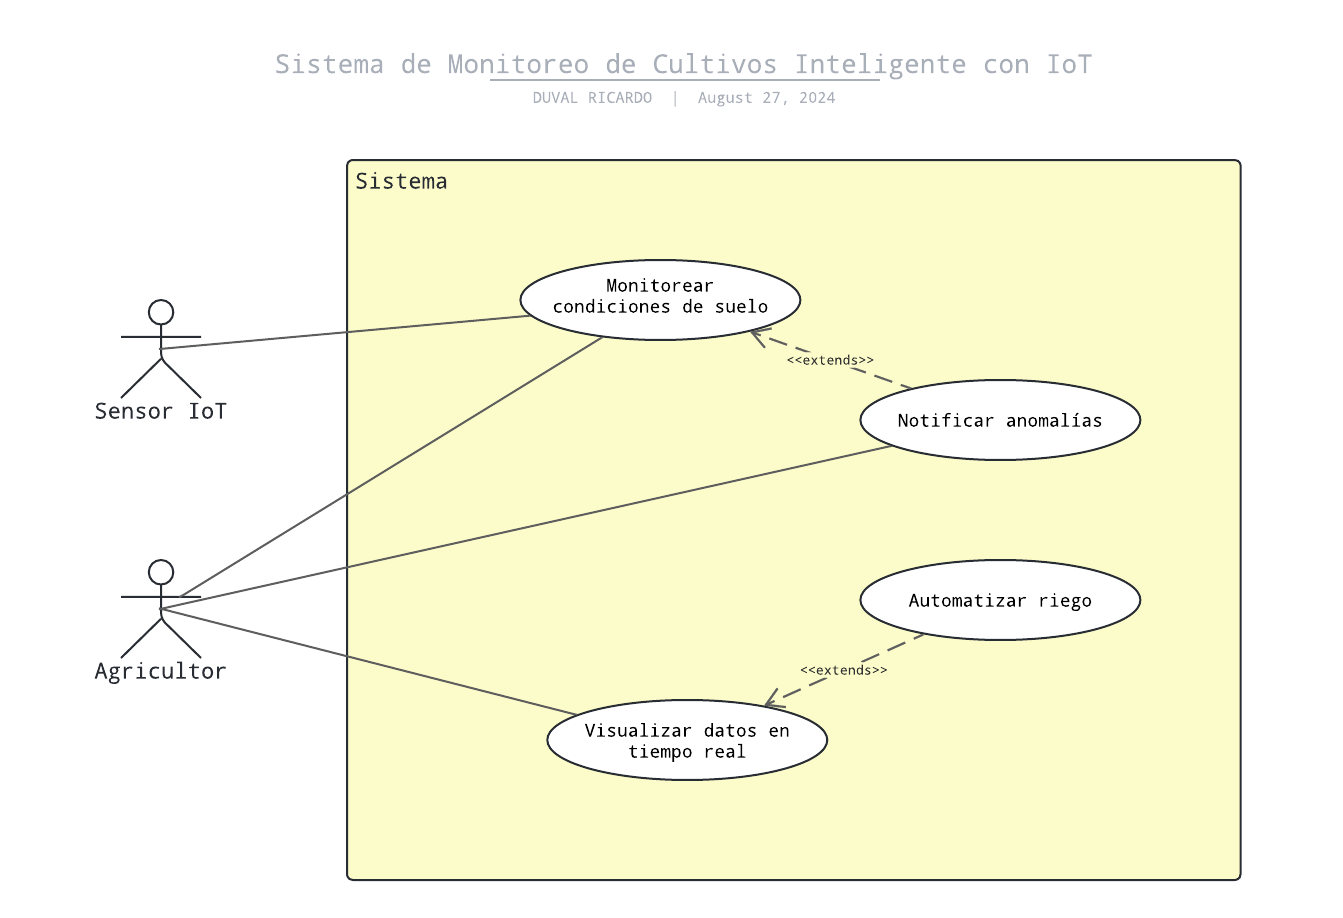
\includegraphics[width=300px]{proyecto001.png} 
	\caption{Diagrama de casos de uso para el Sistema de Monitoreo de Cultivos Inteligente con IoT.}
	\label{fig:cap3_proyecto_001}
\end{figure}

Todos los proyectos que sirvieron para evaluar la extensión están realizados de esta forma, con el objetivo de obtener información lo más apegado a la realidad. Dichos proyectos son trabajos de los estudiantes que presentaran en sus asignaturas respectivas.